%\documentclass[a4paper,11pt,oneside,openright,final,msc,project]{ufmgthesis}
%\documentclass[a4paper,11pt,oneside,openright,msc,project]{ufmgthesis}
\documentclass[a4paper,11pt,oneside,openright,msc,project,hideall]{ufmgthesis}
\usepackage[brazil]{babel}
\usepackage[latin1]{inputenc}
\usepackage[T1]{fontenc}
\usepackage{type1ec}
\usepackage{graphicx}
\ifpdf
	\usepackage{epstopdf}
\fi
\usepackage[
	a4paper,
	portuguese,
	bookmarks=true,
	bookmarksnumbered=true,
	linktocpage,
	colorlinks]{hyperref}
\usepackage{natbib}

\newtheorem{definition}{Defini��o}
\newtheorem{problem}{Problema}

\begin{document}

\ufmgthesis{
	title={Ortogonalidade Aplicada a Regras de Associa��o},
	author={Leandro Souza Costa},
	university={Universidade Federal de Minas Gerais},
	course={Ci�ncia da Computa��o},
	address={Belo Horizonte},
	date={2008-04-16},
	logo={img/brasao.eps},
	advisor={Wagner Meira Jr.}{Ph.~D.}{.},
	member={Marcos Andr� Gon�alves}{Ph.~D.}{.},
	member={Sandra Aparecida de Amo}{Ph.~D.}{Universidade Federal de Uberl�ndia},
	abstract={Resumo}{resumo.tex},
	ack={agradecimentos.tex}
}

\chapter{Introdu��o}

H� muito j� n�o � mais novidade o fato de que vivemos, hoje, na chamada \textbf{Era da Informa��o} (termo cunhado por Daniel Bell, pelo professor em�rito da Universidade de Harvard), que se define pelo r�pido desenvolvimento da tecnologia de informa��o, caracter�stica marcante da \textbf{Sociedade P�s-Industrial}, onde nota-se que mais importante que possuir a informa��o, � saber onde e como encontr�-la.
\par
Ao longo dos anos, o desenvolvimento tecnol�gico fez com que o constante armazenamento de dados se tornasse uma atividade f�cil e barata. A conseq��ncia deste fato � a alimenta��o de enormes bases de dados, o que proporcionou a  necessidade de se pensar em novas solu��es de ger�ncia, manuten��o e, posteriormente, acesso.
\par
Os Sistemas de Gerenciamento de Banco de Dados (\textbf{SGBD}) surgiram como uma solu��o para ger�ncia e manuten��o de bases, com o objetivo de retirar da aplica��o cliente a responsabilidade de gerenciar o acesso, a manipula��o e a organiza��o dos dados. Entretanto, embora os complexos SGBD's tenham se consolidado como eficientes sistemas na ger�ncia de complexos volumes de dados, e tratado com efici�ncia e efic�cia a recupera��o de informa��es em grandes cole��es, da exist�ncia de tais bases surgiu a necessidade de m�todos mais avan�ados de recupera��o de informa��o, como redu��o de volume de dados, extra��o da ess�ncia da informa��o armazenada, descoberta de padr�es em dados brutos, dentre outros.
\par
Como resposta � necessidade dos novos m�todos de recupera��o de informa��o, surgiu o que chamamos hoje de \textbf{Minera��o de Dados}.

\section{Minera��o de Dados}

Minera��o de dados � o resultado de um longo processo de pesquisa e desenvolvimento, considerado uma das mais importantes fronteiras entre bases de dados e sistemas de informa��o e um dos mais promissores desenvolvimentos interdisciplinares na tecnologia da informa��o \citep{Han00}. Podemos defini-la como o conjunto de m�todos n�o triviais de an�lise de dados e extra��o de informa��o potencialmente �til, impl�cita, previamente desconhecida, e suas novas formas de representa��o e visualiza��o \citep{Kumar06, Hand01, PiatetskyF91}.

Falar das solu��es encontradas na minera��o de dados para resolver os problemas citados, (agrupamento, regras associativas, etc). "Minera��o de dados � uma tecnologia usada para revelar informa��o estrat�gica escondida em grandes massas de dados". \\
fonte: http://br.geocities.com/dugimenes/mineracao.htm \\
fonte: http://pt.wikipedia.org/wiki/Minera\%C3\%A7\%C3\%A3o\_de\_dados \\
Citar \cite{Kumar06}. \\
Procurar livros, como \cite{Han00}. \\
http://books.google.com/books?hl=en\&lr=\&id=AfL0t-YzOrEC\&oi=fnd\&pg=PR21\&dq=data+mining\&ots=UuSVuVarG6\&sig=swJzbDeqSGlffWudUjXszg5vNPA\#PPP1,M1

\subsection{Padr�es Freq�entes}

�timo Survey sobre minera��o de padr�es freq�entes (possui descri��o do problema, minera��o de itemsets, espa�o de busca, regras de associa��o, algoritmo apriori fp-growth, etc...): \cite{goethals03survey}.

\subsection{Regras de Associa��o}

Artigo que fala de classifica��o e Regras de Associa��o: \cite{liu98integrating} (CBA)
O Survey tamb�m fala de regras de associa��o: \cite{goethals03survey}.
Artigo do Zaki, que fala tamb�m (CHARM): \cite{zaki99charm}.
Novos algoritmos para descoberta r�pida de regras de associa��o: \cite{DBLP:conf/kdd/ZakiPOL97}.

\section{Ortogonalidade}

Boa fonte para ortogonalidade (termo geral) - wikepedia: http://en.wikipedia.org/wiki/Orthogonal \\
Citar poucos artigos que tratam de ortogonalidade, como ORIGAMI \citep{zaki07origami}, Redundancy-Aware Top-k Patterns \citep{DBLP:conf/kdd/XinCYH06} e Orthogonal Decision Trees \citep{dutta2004orthogonal}. \\
Procurar mais fontes.

\section{Organiza��o do Documento}

�ltimo texto a ser escrito...

\chapter{Algoritmos de Classifica��o}

O artigo \cite{DBLP:conf/icde/ChengYHH07} possui uma se��o dizendo por qu� padr�es frequentes s�o bons para classifica��o.

\section{Fundamentos Te�ricos e Defini��es}

Procurar livros de minera��o de dados e artigos antigos. \\
Falar sobre regras de associa��o. \\
Falar de �rvores de decis�o.

\section{Estrat�gias eager e lazy}

Em \cite{Veloso06Lazy} O Adriano discute bem as duas estrat�gias, procurar mais artigos relacionados. \\
Descrever as duas estrat�gias, e apresentar as vantagens do lazy.

\section{M�tricas de Regras de Associa��o}

Falar sobre similaridade, cobertura, lift, leverage, etc. \\
fonte: http://www.daylight.com/meetings/emug01/Bradshaw/Similarity/YAMS.html \\
fonte: http://wwwai.wu-wien.ac.at/\%7Ehahsler/research/association\_rules/measures.html

\section{Trabalhos Relacionados}

Falar de \cite{DBLP:conf/kdd/KnobbeH06}, que obt�m, de um conjunto de itens, um itemset que particione uma base de dados o mais uniformemente poss�vel.
Falar de \cite{DBLP:conf/icde/LentSW97} ??? artigo que realiza agrupamento de regras de associa��o num espa�o bi-dimensional.
Falar de \cite{DBLP:conf/kdd/XinCYH06}, que extrai top-k padr�es minimizando a redund�ncia de um conjunto de padr�es frequentes.
Falar sobre o ORIGAMI \cite{zaki07origami}.
Falar sobre o lazy \cite{Veloso06Lazy}

\chapter{Padr�es Freq�entes e Ortogonais}
\label{chapter:ortogonalidade}

Como j� foi mencionado na se��o \ref{sec:introducao_padroes}, padr�es freq�entes s�o largamente utilizados em diversas aplica��es na �rea de minera��o de dados, incluindo regras de associa��o, classifica��o, agrupamento, indexa��o, dentre outras. Encontra-se, na literatura, uma grande quantidade de algoritmos de minera��o de padr�es freq�entes que, para muitas aplica��es, produzem resultados satisfat�rios (como os apresentados na se��o \ref{sec:introducao_trabalhos}). Entretanto, grande parte destas solu��es ainda possuem problemas n�o resolvidos.
\par
Uma das raz�es que contribuem para este fato � que, de acordo com a defini��o, qualquer sub-conjunto de um padr�o freq�ente tamb�m � freq�ente, o que faz com que o tamanho do conjunto-solu��o do algoritmo cres�a de maneira explosiva. A introdu��o de conceitos como padr�es fechados ou padr�es maximais ajudou a resolver esta quest�o, por�m, as abordagens existentes minimizam o conjunto-solu��o apenas sob a perspectiva do suporte, n�o considerando a sem�ntica dos dados, o que pode fazer com que padr�es interessantes ao usu�rio sejam retirados da solu��o durante o processo de minimiza��o do resultado.
\par
Outro desafio que ainda persiste na minera��o de padr�es freq�entes � a elimina��o de redund�ncia nos resultados obtidos. Em muitas aplica��es encontramos a necessidade de extrair um pequeno conjunto de padr�es freq�entes que tenham, n�o s� alta signific�ncia, mas tamb�m baixa redund�ncia. A signific�ncia �, em geral, definida pelo contexto da aplica��o. De acordo com \cite{DBLP:conf/kdd/XinCYH06}, alguns estudos recentes t�m se concentrado em como extrair top-$k$ padr�es com alta signific�ncia, e outros em como remover redund�ncia entre padr�es, mas poucos t�m se dedicado a obter sub-conjuntos de alta signific�ncia e baixa redund�ncia ao mesmo tempo.
\par
O objetivo da aplica��o de ortogonalidade no problema da minera��o de padr�es freq�entes � desenvolver uma t�cnica capaz de extrair um sub-conjunto de padr�es com tanto alta signific�ncia quanto baixa redund�ncia entre seus elementos.
\par
%Como j� foi mencionado no cap�tulo \ref{chapter:classificacao}, encontra-se, na literatura, diversos trabalhos relacionados com classifica��o, explorando o problema das mais variadas maneiras, e apresentando modelos diferentes, capazes de se adaptar aos diversos tipos de aplica��es existentes.
%\par
%Paralelamente, a ortogonalidade tem aparecido, em alguns dos �ltimos trabalhos de minera��o de dados, como uma forma de se resolver problemas de redund�ncia em conjuntos de padr�es freq�entes extra�dos de determinada base de dados.
%\par
%A utiliza��o de ortogonalidade para se diminuir a redund�ncia dos conjuntos de padr�es utilizados na gera��o de regras associativas aparece como uma poss�vel forma de se melhorar a efic�cia de tais classificadores. Assim, surge a motiva��o para a aplica��o de m�tricas de ortogonalidade entre padr�es no modelo de classifica��o associativa.
%\par
%Este cap�tulo apresenta as informa��es relacionadas � nova abordagem de classifica��o associativa proposta. Na se��o \ref{sec:ortogonalidade_metricas} ser�o apresentadas as m�tricas de ortogonalidade exploradas, na se��o \ref{sec:ortogonalidade_estrategias} ser�o discutidas as estrat�gias de aplica��o das m�tricas. A se��o \ref{sec:ortogonalidade_classificacao} possui uma discuss�o sobre as formas como a ortogonalidade foi utilizada dentro do modelo de classifica��o, e a se��o \ref{sec:ortogonalidade_origami} apresenta a estrat�gia ORIGAMI e adapta��o desenvolvida para o problema de classifica��o.
 
\section{M�tricas de Ortogonalidade}
\label{sec:ortogonalidade_metricas}

Para se extrair um sub-conjunto de padr�es de alta signific�ncia e baixa redund�ncia em rela��o ao conjunto original de padr�es freq�entes, � necess�rio definir m�tricas que possibilitem a avalia��o dos v�rios conjuntos-solu��o poss�veis. Na literatura, encontramos alguns exemplos de tais m�tricas. Em \cite{DBLP:conf/kdd/XinCYH06} os autores utilizam, em seus experimentos, o complemento do coeficiente de \textbf{Jaccard} \citep{jain88} aplicado � cobertura da base de dados para se obter uma medida de dist�ncia entre dois padr�es: \[D(p_1,p_2) = 1 - \frac{|TS(p_1) \cap TS(p_2)|}{|TS(p_1) \cup TS(p_2)|},\] onde $TS(p)$ � o conjunto de transa��es cobertas pelo padr�o $p$.
\par
Em \cite{zaki07origami} os autores discutem diferentes m�tricas de similaridade entre grafos, incluindo, al�m do coeficiente de \textbf{Jaccard}: \[sim(G_a, G_b) = \frac{|t(G_a) \cap t(G_b)|}{|t(G_a) \cup t(G_b)|},\] uma m�trica de dist�ncia para grafos baseada no m�ximo sub-grafo comum \citep{bunke98}: \[sim_{mc}(G_1, G_2) = \frac{|G_{mc}|}{max(|G_1|,|G_2|)},\] onde $G_{mc}$ � o maior sub-grafo comum entre $G_1$ e $G_2$.
\par
A principal caracter�sticas destas m�tricas � que elas foram desenvolvidas para avalia��o de pares de padr�es, e n�o aplic�veis em conjuntos de tamanho maior que $2$. No nosso caso, estamos interessados em m�tricas que definem a ortogonalidade de conjuntos de qualquer tamanho. Nas pr�ximas sub-se��es apresentaremos tr�s m�tricas de ortogonalidade propostas e indicadas para o problema da classifica��o associativa.

%A aplica��o da ortogonalidade no modelo de classifica��o associativa tem como principal objetivo a diminui��o de redund�ncia no conjunto de regras geradas durante a fase de treinamento. Para tanto, podem ser  naO objetivo da ortogonalidade � diminuir o n�mero de padr�es utilizados para gerar as regras de associa��o. Logo, a sua utiliza��o ....

\subsection{Estrutura dos Padr�es}
\label{sec:ortogonalidade_metricas_estrutura}

Considerando a estrutura dos padr�es, ou seja, a seq��ncia de itens pelos quais s�o definidos, dizemos que dois padr�es s�o ortogonais se eles n�o possuem itens em comum, ou seja, pode-se dizer que os padr�es $ABC$ e $DEF$ s�o ortogonais, mas $ABC$ e $CDE$ n�o o s�o, j� que o item $C$ est� presente nos dois padr�es. O mesmo pode ser aplicado a conjuntos maiores, por exemplo, os padr�es $AB$, $CD$ e $EF$ s�o ortogonais, mas os padr�es $AB$, $BC$ e $CD$ n�o o s�o.
\par
Entretanto, a simples informa��o de que um determinado conjunto de padr�es � ortogonal ou n�o � insuficiente para que um poss�vel conjunto-solu��o seja avaliado. Para tanto, � preciso desenvolver uma m�trica dada por uma fun��o $\F \rightarrow \left[0, 1\right]$ que forne�a a medida de ortogonalidade do conjunto.
\par
Uma forma de se obter esta medida, � analisar os itens dos padr�es. Sabemos que dois padr�es s�o ortogonais se eles n�o compartilham itens, ou seja, a presen�a de um mesmo item em mais de um padr�o do conjunto, intuitivamente, deve contribuir de maneira negativa para a medida de ortogonalidade do mesmo. A m�trica de ortogonalidade baseada na estrutura dos padr�es associa pesos aos itens, de modo que quanto maior a sua popularidade, menor ser� o seu peso. O resultado � dado pela m�dia dos pesos de todos os itens que fazem parte dos padr�es do conjunto.
\par
Seja $\I$ um conjunto de itens, $\D$ uma base de dados de transa��es em $\I$, $\F$ o conjunto de padr�es freq�entes em $\D$, e $\Fl$ um sub-conjunto de $\F$ ($\Fl \subseteq \F$). Chamamos de $\Il \subseteq \I$ o sub-conjunto itens que aparecem em, pelo menos, um dos padr�es de $\Fl$. Para cada item $i \subseteq \Il$ � dado um peso: \[w_i = \frac{|\Fl|-|\Fli|}{|\Fl|-1},\] onde $\Fli \subseteq \Fl$ � o sub-conjunto de padr�es de $\Fl$ que cont�m o item $i$.
\par
De acordo com esta express�o, se o conjunto possui quatro padr�es, e um item $i$ est� presente em apenas um deles, o valor do seu peso $w_i$ � equivalente a $1$. Se o item estiver presente em $3$ padr�es do conjunto, o peso $w_i$ ser� $\frac{1}{3}$. Itens compartilhados por todos os padr�es t�m peso igual a $0$.
\par
Finalmente, a ortogonalidade baseada na estrutura dos padr�es do conjunto � dada por: \[O_e = \frac{\sum_{i \subseteq \Il} w_i}{|\Il|}.\]
\par
Como exemplo, suponha um conjunto de itens $\I = \left\{A, B, C, D, E \right\}$ e um conjunto de padr�es: $\F = \left\{ AB, ABC \right\}$. Na tabela \ref{tab:item_w1} encontramos valor do peso de cada item, de acordo com a express�o apresentada. Os itens $D$ e $E$ n�o possuem pesos, pelo fato de n�o serem encontrados nos padr�es.

\begin{table}[htbp]
	\centering
		\begin{tabular}{|c|c|}
		\hline
		Itens	& Pesos	\\
		\hline
		$A$	& $0$	\\
		\hline
		$B$	& $0$	\\
		\hline
		$C$	& $1$	\\
		\hline
		$D$	& $-$	\\
		\hline
		$E$	& $-$	\\
		\hline
		\end{tabular}		
	\caption{Pesos dos Itens para Ortogonalidade Baseada na Estrutura dos Padr�es (1)}
	\label{tab:item_w1}
\end{table}

Como podemos ver, o item $C$ � o �nico que faz parte de apenas um padr�o, portanto, � associado o peso $1$ para este item. Os outros dois itens ($A$ e $B$) s�o encontrados nos dois padr�es, e por isso, possuem peso $0$. De acordo com a express�o de ortogonalidade, m�dia destes valores nos d� a medida de ortogonalidade do conjunto: $O_e = 0,33$. Agora, suponha que seja inserido o novo padr�o $BCD$ ao conjunto ($\F = \left\{ AB, ABC, BCD \right\}$). A tabela \ref{tab:item_w2} possui os novos pesos para cada item.

\begin{table}[htbp]
	\centering
		\begin{tabular}{|c|c|}
		\hline
		Itens	& Pesos	\\
		\hline
		$A$	& $0,5$	\\
		\hline
		$B$	& $0$	\\
		\hline
		$C$	& $0,5$	\\
		\hline
		$D$	& $1$	\\
		\hline
		$E$	& $-$	\\
		\hline
		\end{tabular}		
	\caption{Pesos dos Itens para Ortogonalidade Baseada na Estrutura dos Padr�es (2)}
	\label{tab:item_w2}
\end{table}

Note que o novo padr�o possui um novo item ($D$) que antes n�o era encontrado no conjunto. A inser��o de $BCD$ fez com que o peso de $A$ aumentasse, visto que este item n�o faz parte do padr�o. J� o peso de $B$ continuou o mesmo, e o novo item $D$ entrou no conjunto com peso $1$. Assim, a ortogonalidade do novo conjunto � $O_e = 0,5$.

%Dois padr�es s�o similares se possuem itens em comum, logo, dois padr�es s�o ortogonais se n�o possuem itens em comum. Mostrar exemplo: AB e CD s�o mais ortogonais que AB e BC. Fazer figura do exemplo.

\subsection{Cobertura de Transa��es}
\label{sec:ortogonalidade_metricas_transacoes}

Considerando o espa�o de transa��es, dizemos que dois padr�es s�o ortogonais se eles cobrem �reas diferentes da base de dados, ou seja, se n�o existem sobreposi��es nas coberturas de cada padr�o do conjunto.
\par
Na figura \ref{fig:covex1} temos uma representa��o de uma base de dados, e os conjuntos de transa��es cobertas por tr�s padr�es ($X$, $Y$ e  $Z$). As transa��es que fazem parte das �reas $T_X$, $T_Y$ e $T_Z$ s�o cobertas por apenas um dos padr�es ($X$, $Y$ e $Z$ respectivamente). As transa��es de $T_{XY}$ s�o cobertas por $X$ e $Y$, e as transa��es de $T_{XYZ}$ s�o cobertas pelos tr�s padr�es do exemplo. Se precisamos de padr�es que cobrem diferentes �reas da base de dados, ent�o n�s estamos interessados em maximizar $T_X$, $T_Y$ e $T_Z$, no caso do exemplo.

\begin{figure}
\centering
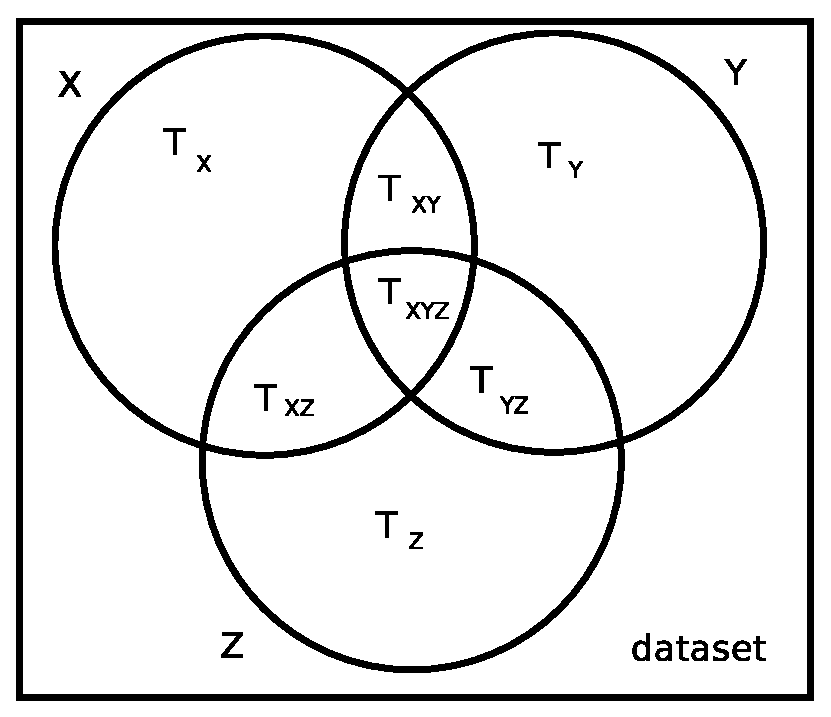
\includegraphics[width=0.5\textwidth]{img/coverage}
\caption{Visualiza��o de Cobertura de Transa��es na Base de Dados}
\label{fig:covex1}
\end{figure}

%\begin{figure}
%\centering
%\begin{picture}(180,180)
%\linethickness{0.075mm}
%\thicklines
%external frame
%\multiput(0, 0)(180, 0){2}{\line(0, 1){180}}
%\multiput(0, 0)(0, 180){2}{\line(1, 0){180}}

%circle X
%\put(90,90){\circle{170}}
%\framebox[100, 100]{teste}
%\put(-50,50){\frame{\circle{100}}
%\end{picture}
%\caption{Visualiza��o de Cobertura de Transa��es na Base de Dados}
%\end{figure}

A m�trica de ortogonalidade baseada em cobertura de transa��es pode ser calculada de maneira an�loga � relacionada com a estrutura, sendo que, neste caso, os elementos que possuem pesos a serem calculados s�o as transa��es cobertas pelos padr�es, e n�o os seus itens.
\par
Seja $\I$ um conjunto de itens, $\D$ uma base de dados de transa��es em $\I$, $\F$ o conjunto de padr�es freq�entes em $\D$, e $\Fl$ um sub-conjunto de $\F$ ($\Fl \subseteq \F$). Chamamos de $\Dl \subseteq \D$ o sub-conjunto transa��es cobertas por, pelo menos, um dos padr�es de $\Fl$. Para cada transa��o $t \subseteq \Dl$ � dado um peso: \[w_t = \frac{|\Fl| - |\Flt|}{|\Fl| - 1},\] onde $\Flt$ � o sub-conjunto de padr�es de $\Fl$ que cobrem a transa��o $t$.
\par
De acordo com esta express�o, se n�s tivermos $4$ padr�es, e uma transa��o $t$ coberta por apenas um deles, ent�o o seu peso $w_t$ ser� $1$. Se esta transa��o for coberta por dois padr�es do conjunto, o valor de $w_t$ ser� $\frac{1}{2}$. As transa��es cobertas por todos os padr�es do conjunto ter�o peso igual a $0$.
\par
A ortogonalidade baseada em cobertura de transa��es do conjunto � dada por: \[O_t = \frac{\sum_{t \subseteq \Dl} w_t}{|\Dl|}.\]
\par
Suponha uma base de dados $\D = \left\{ A, ABCD, BCDE, CDEF \right\}$, e um conjunto de padr�es $\F = \left\{ AB, BC, CD \right\}$. Na tabela \ref{tab:transacao_w1} encontramos valor do peso de cada transa��o, de acordo com a express�o apresentada. A transa��o $A$ n�o possui peso, pelo fato de n�o ser coberta por nenhum dos padr�es.

\begin{table}[htbp]
	\centering
		\begin{tabular}{|c|c|}
		\hline
		Transa��es	& Pesos	\\
		\hline
		$A$		& $-$	\\
		\hline
		$ABCD$		& $0$	\\
		\hline
		$BCDE$		& $0,5$	\\
		\hline
		$CDEF$		& $1$	\\
		\hline
		\end{tabular}		
	\caption{Pesos das Transa��es para Ortogonalidade Baseada na Cobertura de Transa��es}
	\label{tab:transacao_w1}
\end{table}

A transa��o $CDEF$ � a �nica coberta por apenas um padr�o do conjunto, portanto, � associado o peso $1$ para ela. A transa��o $BCDE$ � coberta por dois padr�es, portanto, recebe o peso $0,5$, e a transa��o $ABCD$ recebe o peso $0$, j� que ela � coberta por todos os padr�es do conjunto. A m�dia dos pesos das transa��es nos d� o valor da ortogonalidade do conjunto: $O_t = 0,5$.

\subsection{Cobertura de Classes}
\label{sec:ortogonalidade_metricas_classes}

As duas m�tricas de ortogonalidade apresentadas nas se��es \ref{sec:ortogonalidade_metricas_estrutura} e \ref{sec:ortogonalidade_metricas_transacoes} est�o relacionadas apenas com os padr�es e as transa��es da base, e podem ser utilizadas em qualquer tipo de aplica��o. J� a m�trica apresentada nesta se��o � voltada diretamente para o problema da classifica��o, pois est� relacionada �s classes das transa��es cobertas pelos padr�es do conjunto.
\par
A motiva��o para esta m�trica est� calcada na seguinte considera��o: Dois padr�es s�o ortogonais se s�o encontrados em transa��es de classes distintas na base de dados, ou seja, os conjuntos de transa��es cobertas por cada um dos padr�es n�o devem possuir classes em comum.
\par
A m�trica de cobertura de classes pode ser calculada de maneira an�loga �s relacionadas m�tricas de similaridade entre padr�es e cobertura de transa��es, sendo que, neste caso, os elementos que possuem pesos a serem calculados s�o as classes existentes nas transa��es cobertas pelos padr�es.
\par
Seja $\I$ um conjunto de itens, $\D$ uma base de dados de transa��es em $\I$, $\F$ o conjunto de padr�es freq�entes em $\D$, e $\Fl$ um sub-conjunto de $\F$ ($\Fl \subseteq \F$). Chamamos de $\Dl \subseteq \D$ o sub-conjunto transa��es cobertas por, pelo menos, um dos padr�es de $\Fl$. Seja $\C$ um conjunto de classes associadas �s transa��es de $\D$. Chamamos de $\Cl \subseteq \C$ o sub-conjunto de classes associadas �s transa��es de $\Dl$. Para cada classe $c \subseteq \Cl$ � dado um peso: \[w_c = \frac{|\Fl| - |\Flc|}{|\Fl| - 1},\] onde $\Flc$ � o sub-conjunto de padr�es de $\Fl$ que cobrem uma quantidade de transa��es de classe $c \subseteq \Cl$ maior que $90\%$ da m�dia esperada \footnote{Dado um conjunto de transa��es $\Dlc$ onde todas as transa��es possuem a classe $c$ e um conjunto de padr�es $\Fl$ em $\Dlc$, a cobertura esperada de cada padr�o para a classe $c$ � $\frac{|\Dlc|}{|\Fl|}$ (considerando que todos os padr�es s�o independentes, ou seja, ortogonais).}.
\par
De acordo com esta express�o, se n�s temos 4 padr�es, e uma classe $c$ que aparece em transa��es cobertas por apenas um deles, ent�o o seu peso $w_c$ ser� $1$. Se esta classe aparece em transa��es cobertas por dois padr�es do conjunto de maneira balanceada (por exemplo, $50\%$ das  transa��es da classe aparece em um dos padr�es, e o $50\%$ restantes no outro), o valor de $w_c$ ser� $\frac{1}{2}$. As classes que aparecem por igual em transa��es cobertas por todos os padr�es do conjunto ter�o peso igual a $0$.
\par
Por fim, a ortogonalidade baseada em cobertura de classes � dada por: \[O_c = \frac{\sum_{c \subseteq \Cl} w_c}{|\Cl|}.\]
\par
Suponha uma base de dados $\D$ em que as transa��es respectivas classes s�o encontradas na tabela \ref{tab:classe_db}.

\begin{table}[htbp]
	\centering
		\begin{tabular}{|c|c|}
		\hline
		Transa��es	& Classes	\\
		\hline
		$ABCD$		& $1$		\\
		\hline
		$ACD$		& $1$		\\
		\hline
		$BCDE$		& $1$		\\
		\hline
		$BDEF$		& $2$		\\
		\hline
		$CDE$		& $2$		\\
		\hline
		$CEF$		& $2$		\\
		\hline
		\end{tabular}		
	\caption{Base de Dados de Transa��es e Classes}
	\label{tab:classe_db}
\end{table}

Suponha um conjunto de padr�es $\F = \left\{AB, CD, EF \right\}$. Os pesos de cada classe, de acordo com a express�o apresentada, s�o encontrados na tabela \ref{tab:classe_w1}.

\begin{table}[htbp]
	\centering
		\begin{tabular}{|c|c|}
		\hline
		Classes	& Pesos	\\
		\hline
		$1$	& $1$	\\
		\hline
		$2$	& $0,5$	\\
		\hline
		\end{tabular}		
	\caption{Pesos das Classes para Ortogonalidade Baseada na Cobertura de Classes}
	\label{tab:classe_w1}
\end{table}

Como pode ser visto na tabela \ref{tab:classe_db}, a classe $1$ � coberta uma vez pelo padr�o $AB$ (transa��o $ABCD$, e tr�s vezes pelo padr�o $CD$ (transa��es $ABCD$, $ACD$ e $BCD$), totalizando $4$ coberturas. Como o conjunto de padr�es possui tamanho $3$, considerando que todos os padr�es sejam independentes, espera-se que a cobertura de classes seja homog�nea, ou seja, que cada padr�o cubra $4/3$ transa��es de cada classe. De acordo com a express�o apresentada, consideramos $\Flc$ o conjunto de padr�es que cobrem uma quantidade de transa��es da classe $c$ maior que $90\%$ da m�dia esperada (neste caso, $1,2$). Do nosso conjunto de padr�es, o �nico que satisfaz esta premissa � $CD$, que ocorre em $3$ transa��es da classe $1$. Logo, o peso dessa classe � $1$.
\par
J� a classe $2$ � coberta duas vezes pelo padr�o $CD$, e duas vezes pelo padr�o $EF$, logo, tamb�m possui cobertura esperada igual a $4/3$. Entretanto, os dois padr�es possuem cobertura desta classe acima de $90\%$ da m�dia esperada, logo, o peso dessa classe � $0,5$. A m�dia dos pesos das classes nos d� o valor da ortogonalidade do conjunto: $O_c = 0,75$.

\subsection{Utiliza��o das M�tricas}
\label{sec:ortogonalidade_estrategias}

Ap�s a introdu��o das m�tricas, � necess�rio definir como elas ser�o utilizadas para se obter a medida de ortogonalidade do conjunto. Na literatura, encontramos algumas estrat�gias interessantes.
\par
Em \cite{zaki07origami} � utilizada uma medida de ortogonalidade aplic�vel a pares de padr�es. Os autores optaram por utilizar, como m�trica do conjunto, o valor da ortogonalidade entre os seus dois elementos mais similares.
\par
Em \cite{DBLP:conf/kdd/XinCYH06} os autores utilizaram m�tricas de signific�ncia aplic�veis a padr�es e m�tricas de redund�ncia aplic�veis a pares de padr�es. O valor da fun��o que compreende as duas m�tricas � obtido pela soma das signific�ncias de cada padr�o do conjunto menos a m�dia das redund�ncias existentes entre todos os pares de padr�es.
\par
Neste trabalho, duas solu��es foram implementadas. A primeira delas � baseada na medida de ortogonalidade do conjunto, onde aplicamos as m�tricas apresentadas na se��o \ref{sec:ortogonalidade_metricas} considerando todo o conjunto-solu��o. A segunda � baseada na solu��o proposta por \cite{DBLP:conf/kdd/XinCYH06} - as m�tricas s�o aplicadas somente a pares de padr�es, e a ortogonalidade do conjunto � obtida por meio da m�dia das ortogonalidades entre todos os pares poss�veis.
\par
� f�cil perceber que as m�tricas propostas nas se��es \ref{sec:ortogonalidade_metricas_estrutura} e \ref{sec:ortogonalidade_metricas_transacoes} e \ref{sec:ortogonalidade_metricas_classes} s�o equivalentes ao complemento do coeficiente de Jaccard quando aplicadas a conjuntos de dois padr�es. Tomando a m�trica baseada na estrutura dos padr�es como exemplo, temos que a ortogonalidade do conjunto � dada pela express�o: \[O_e = \frac{\sum_{i \subseteq \Il} \left( \frac{|\Fl| - |\Fli|}{|\Fl| - 1} \right)}{|\Il|}.\] Nos casos em que o conjunto de possui necessariamente dois padr�es: \[ O_e = \frac{\sum_{i \subseteq \Il} (2 - |\Fli|)}{|\Il|}.\] Analisando a express�o acima, temos que $|\Il|$ corresponde ao tamanho do conjunto de itens encontrados nos dois padr�es, ou seja, \[|\Il| = |p_1 \cup p_2|,\] onde $\Fl = \left\{p1, p2 \right\}$, e a parcela $(2 - |\Fli|)$ ter� valor $1$ para itens que est�o presentes em apenas um dos padr�es, e $0$ para itens presentes nos dois padr�es, ou seja, \[\sum_{i \subseteq \Il} (2 - |\Fli|) = |p_1 \cup p_2| - |p_1 \cap p_2|.\] Logo, a m�trica de ortogonalidade baseada na estrutura dos padr�es, quando aplicada par-a-par, � dada pela seguinte express�o: \[O_e = 1 - \frac{\sum_{p_1, p_2 \subseteq \Fl, p_1 \neq p_2} \frac{|p_1 \cap p_2|}{|p_1 \cup p_2|}}{\frac{|\Fl| \times (|\Fl|-1)}{2}}.\]
\par
A m�trica de ortogonalidade baseada em cobertura de transa��es, quando aplicada par-a-par, � dada pela seguinte express�o: \[O_t = 1 - \frac{\sum_{p_1, p_2 \subseteq \Fl, p_1 \neq p_2} \frac{|\Dl_{p1} \cap \Dl_{p2}|}{|\Dl_{p1} \cup \Dl_{p2}|}}{\frac{|\Fl| \times (|\Fl|-1)}{2}},\] onde $\Dl_p$ � o sub-conjunto de transa��es cobertas pelo padr�o $p$.
\par
A m�trica de ortogonalidade baseada em cobertura de classes, quando aplicada par-a-par, � dada pela seguinte express�o: \[O_c = 1 - \frac{\sum_{p_1, p_2 \subseteq \Fl, p_1 \neq p_2} \frac{|\Cl_{p1} \cap \Cl_{p2}|}{|\Cl_{p1} \cup \Cl_{p2}|}}{\frac{|\Fl| \times (|\Fl|-1)}{2}},\] onde $\Cl_p$ � o sub-conjunto de classes cujas transa��es s�o cobertas pelo padr�o $p$ $90\%$ acima da m�dia esperada.

%Breve introdu��o, falar sobre m�tricas utilizadas por \cite{DBLP:conf/kdd/XinCYH06} e \cite{zaki07origami}.

%\subsection{Ortogonalidade por conjunto}

%Apresentar e discutir as express�es: \\
%Similaridade: Express�o que d� um peso para cada item encontrado nos padr�es do conjunto; \\
%Cobertura de Transa��es: Express�o que d� um peso para cada transa��o coberta pelo conjunto de padr�es; \\
%Cobertura de Classes: Express�o que d� um peso para cada classe encontrada nas transa��es cobertas pelos padr�es.

%\subsection{Ortogonalidade Par-a-par}

%Discutir as express�es par a par (similaridade pode ser dada por interse��o sobre uni�o de elementos, ortogonalidade pode ser dada por 1 - similaridade): \\
%Ortogonalidade por itens: Quantidade de itens que aparecem em apenas um dos padr�es / quantidade de itens que aparecem nos dois padr�es. \\
%Ortogonalidade por cobertura de transa��es: Quantidade de transa��es cobertas por apenas um dos padr�es / quantidade de transa��es cobertas pelos dois padr�es. \\
%Ortogonalidade por cobertura de classes: Mais complicado: Ortogonalidade � a m�dia das raz�es entre a diferen�a das coberturas e a maior cobertura de cada classe. 

\section{Classifica��o Associativa e Ortogonalidade}
\label{sec:ortogonalidade_classificacao}

Como j� foi dito na se��o \ref{sec:introducao_objetivos}, a utiliza��o da ortogonalidade no problema da classifica��o associativa tem como objetivo aumentar a efetividade das classifica��es, como conseq��ncia da diminui��o da redund�ncia e da ambig�idade das regras. Uma das formas de se fazer isso seria aplicar ortogonalidade no conjunto de regras geradas pelo classificador. Dessa forma, seria poss�vel extrair, de todo o conjunto de regras obtidas, apenas um sub-conjunto representativo de regras com alta signific�ncia e baixa redund�ncia, e a partir destas, realizar a classifica��o das inst�ncias de teste.
\par
Esta proposta � apresentada em \cite{DBLP:conf/kdd/XinCYH06}, onde � discutido utiliza��o de ortogonalidade aplicada a \textit{prefetch} de blocos de acesso a disco. Os autores consideram a similaridade de duas regras igual a $0$ quando os termos conseq�entes s�o diferentes, e igual ao coeficiente de Jaccard aplicado aos termos antecedentes quando os conseq�entes s�o iguais.
\par
� poss�vel aplicar este modelo no problema da classifica��o associativa. Nesse caso, seria considerado como m�trica de ortogonalidade entre duas regras o valor m�ximo ($1$) se as classes para as quais elas apontam s�o diferentes, e o valor inversamente proporcional ao coeficiente de Jaccard (ou alguma outra m�trica qualquer) aplicado aos termos antecedentes se as classes para as quais elas apontam s�o iguais. Dessa forma, estar�amos gerando todas as regras poss�veis, a partir do conjunto de padr�es freq�entes obtidos por meio de um determinado suporte, e extraindo um sub-conjunto que consiste apenas das mais representativas, para ent�o realizar a classifica��o da inst�ncia de teste.
\par
Neste trabalho, por�m, optamos por aplicar a ortogonalidade n�o ao conjunto de regras geradas, mas sim ao conjunto de padr�es utilizados para gerar as regras. A id�ia � gerar regras a partir de um sub-conjunto dos padr�es freq�entes obtidos, que consiste apenas dos padr�es ortogonais. A principal diferen�a desta abordagem, em rela��o � anterior, � que as m�tricas de ortogonalidade s�o aplicadas apenas aos termos antecedentes - os padr�es, ou seja, as classes n�o s�o consideradas.
\par
As tr�s m�tricas descritas na se��o \ref{sec:ortogonalidade_metricas} foram utilizadas neste trabalho. A m�trica baseada na estrutura dos padr�es foi utilizada com o objetivo de se encontrar um sub-conjunto de padr�es que represente bem todo o conjunto de padr�es freq�entes. Por ser uma m�trica que considera o conjunto de itens, ela se aplica ao espa�o dos padr�es, n�o considerando a sua rela��o com as transa��es da base. Neste caso, estamos interessados em diminuir, principalmente, a redund�ncia das regras, ou seja, n�o gerar regras com um alto n�vel de similaridade entre os termos antecedentes.
\par
A cobertura de transa��es foi utilizada com o objetivo de se encontrar padr�es ortogonais no espa�o de transa��es. Com esta m�trica, espera-se obter um sub-conjunto de padr�es que cobrem a base de dados com o m�nimo de sobreposi��es poss�vel, ou seja, que as regras geradas por cada um destes padr�es apontem para transa��es distintas da base. A inten��o, neste caso, � diminuir a ambig�idade das regras, al�m da redund�ncia.
\par
A cobertura de classes � uma m�trica definida especialmente para o problema da classifica��o, j� que ela considera as classes das transa��es da base de treinamento para definir o conjunto de padr�es ortogonais. Esta m�trica � uma adapta��o da cobertura de transa��es, visto que ela tamb�m est� centrada na base de dados. A diferen�a � que, ao contr�rio da anterior, esta m�trica analisa as classes, e n�o as transa��es cobertas pelos padr�es. A motiva��o � que n�o basta extrair padr�es que cobrem transa��es distintas da base de dados se estas transa��es possuem classes coincidentes. Esta m�trica tenta garantir que as regras geradas pelo conjunto-resultado de padr�es apontem para classes distintas. A inten��o, como na m�trica anterior, � diminuir a ambig�idade das regras, al�m da redund�ncia.

%Falar sobre como utilizar o conceito de ortogonalidade em algoritmos de regras de associa��o:
%Ortogonalidade por itens: Motiva��o: Encontrar um conjunto de padr�es ortogonais que representem bem todo o conjunto de padr�es freq�entes, e que gere regras n�o redundantes;
%Ortogonalidade por cobertura de transa��es: Encontrar um conjunto de padr�es que cubram �res ortogonais, e dessa forma, distintas da base de dados, diminuindo a redund�ncia de informa��es durante a gera��o das regras, e mais que isso, diminuindo a possibilidade de encontrar regras redundantes;
%Ortogonalidade por cobertura de classes: Encontrar um conjunto de padr�es que aparecem em transa��es de classes distintas, ou seja, padr�es que apontam para classes distintas. A id�ia � gerar regras n�o redundantes, e obter a classifica��o das regras de maior peso no ranking.

\subsection{Utiliza��o de Ortogonalidade no LAC}

O \textbf{LAC} (\textit{Lazy Associative Classifier}) � uma implementa��o da abordagem \textit{lazy} proposta em \cite{Veloso06Lazy}. A abordagem de classifica��o associativa \textit{lazy} obt�m o conjunto de regras de associa��o relacionadas a cada inst�ncia de teste separadamente. Para tanto, ela cria uma proje��o da base de treinamento apenas com as transa��es que possuem itens em comum com a inst�ncia de teste. A partir desta proje��o, a abordagem obt�m um conjunto de padr�es freq�entes, de acordo com determinado suporte fornecido pelo usu�rio, e com estes padr�es, gera as regras de associa��o utilizadas durante a tarefa de classifica��o.
\par
A ortogonalidade pode ser utilizada de v�rias maneiras no \textit{lazy}, por exemplo, � poss�vel extrair, \textit{apriori}, o conjunto de itens ortogonais da base de treinamento, considerando cobertura de transa��es, ou cobertura de classes, e, para cada inst�ncia de teste, obter a proje��o da base de treinamento considerando apenas os itens que fazem parte do conjunto ortogonal. Esta seria uma boa op��o para diminuir o espa�o de busca durante a obten��o do conjunto de padr�es freq�entes nos casos em que as bases de dados s�o muito densas.
\par
Uma outra maneira seria extrair o conjunto de itens ortogonais, n�o de toda a base de treinamento, mas sim de cada inst�ncia no momento do teste. Entretanto, tanto esta forma quanto a anterior ainda possibilitaria a gera��o de conjuntos de regras redundantes, j� os itens obtidos, mesmo mantendo a caracter�stica de ortogonalidade entre si, poderiam gerar padr�es similares.
\par
Sendo assim, a forma escolhida neste trabalho foi continuar utilizando todos os itens da inst�ncia de teste para gerar a proje��o da base. A partir destes, obter o conjunto de padr�es freq�entes e ent�o, extrair o sub-conjunto de padr�es ortogonais, com os quais s�o geradas as regras de associa��o.

\subsection{Heur�stica de Obten��o de Conjuntos Ortogonais}

O problema de se encontrar o sub-conjunto de padr�es com maior m�trica de ortogonalidade, dado o conjunto de padr�es freq�entes, � n�o polinomial, visto que todas as combina��es de todos os tamanhos poss�veis devem ser testadas para se chegar ao resultado final. Portanto, foi desenvolvida uma heur�stica gulosa que inicia com um conjunto ortogonal de dois elementos, e iterativamente, tenta obter um novo conjunto com um elemento a mais, acrescentando padr�es candidatos e realizando modifica��es para que a m�trica de ortogonalidade seja maximizada.
\par
Esta abordagem � semelhante ao que foi proposto em \cite{zaki07origami}. Este artigo apresenta um algoritmo que considera o conjunto de padr�es freq�entes como um grafo em que cada v�rtice representa um padr�o, e uma aresta entre dois v�rtices representa a similaridade entre os padr�es. No entanto, s� s�o representadas as arestas que possuem similaridade menor que $\alpha$ (par�metro do algoritmo). O objetivo da heur�stica � encontrar um clique de tamanho m�ximo neste grafo. Para tanto, o algoritmo escolhe um v�rtice aleatoriamente e o adiciona no conjunto-solu��o. Ap�s este passo, o algoritmo passa a visitar os vizinhos dos v�rtices que j� fazem parte da solu��o, escolhendo sempre o melhor candidato para adicionar ao conjunto, at� que n�o haja mais v�rtices para se adicionar.
\par
No nosso caso, n�o utilizamos o par�metro $\alpha$, limite inferior para a m�trica de ortogonalidade. Sendo assim, todos os padr�es s�o candidatos ao conjunto-resultado. A obten��o do conjunto ortogonal de padr�es � realizada de forma iterativa, onde no in�cio da execu��o, o algoritmo inicializa o conjunto-solu��o com apenas um elemento, e a m�trica de ortogonalidade do conjunto com o valor $0$ (zero), e ent�o come�a o ciclo de itera��es em que, a cada etapa:

\begin{enumerate}
	\item Um novo elemento � inclu�do ao conjunto;
	\item � realizada uma busca por todo o conjunto de padr�es que n�o fazem parte do conjunto-solu��o. Durante este procedimento, cada padr�o verificado � inclu�do na solu��o, substituindo, neste conjunto, o elemento que mais se assemelha �quele. Se a m�trica de ortogonalidade do conjunto melhorou, o algoritmo mant�m a troca. Se n�o, a troca � desfeita, e o pr�ximo padr�o da seq��ncia � verificado;
	\item Ao final do processo, o algoritmo compara a m�trica de ortogonalidade obtida com a m�trica do conjunto anterior (que possu�a um elemento a menos). Se a m�trica se manteve, ou melhorou, o algoritmo mant�m o novo conjunto como solu��o, e volta ao in�cio do ciclo. Se n�o, o algoritmo termina o ciclo, e o conjunto anterior � dado como resultado.
\end{enumerate}

A ordem como o algoritmo percorre o conjunto de padr�es em cada itera��o possui uma grande influ�ncia no algoritmo, pois um novo padr�o verificado s� far� parte do conjunto solu��o se a ortogonalidade do novo conjunto for maior que a do antigo, logo, em caso de empate, os primeiros padr�es ter�o prefer�ncia sobre os �ltimos. Cinco formas diferentes de ordena��o do conjunto de padr�es freq�entes foram implementadas:

\begin{enumerate}
	\item Ordena��o lexicogr�fica crescente;
	\item Ordena��o lexicogr�fica decrescente;
	\item Ordena��o por tamanho crescente;
	\item Ordena��o por tamanho decrescente;
	\item Nenhuma ordena��o.
\end{enumerate}

As ordena��es lexicogr�ficas foram utilizadas para se diminuir a dist�ncia entre dois padr�es da seq��ncia, fazendo com que a modifica��o do conjunto-solu��o seja realizada de forma suave. Espera-se que, neste caso, a diferen�a estrutural entre dois padr�es consecutivos do conjunto durante cada itera��o seja a menor poss�vel. As ordena��es por tamanho foram utilizas para dar prioridade, hora aos maiores padr�es (ordena��o decrescente), hora aos menores padr�es (ordena��o crescente).

O pseudo-c�digo do algoritmo de classifica��o associativa baseada em ortogonalidade \textbf{OLAC} (\textit{Orthogonal Lazy Assiciative Classifier}) pode ser visto no algoritmo \ref{alg:olac}.\

\begin{algorithm}
\caption{OLAC}
\label{alg:olac}
\begin{algorithmic}[1]

\REQUIRE $\D, \sigma$
\STATE $\F \leftarrow FindFrequentPatterns (\D, \sigma)$
\STATE $Sort (\F)$
\STATE $\Or \leftarrow GetFirstAvailablePattern (\F)$
\REPEAT
	\STATE $rate \leftarrow GetOrthogonalityRate (\Or)$
	\STATE $\Or_{try} \leftarrow \Or \cup GetFirstAvailablePattern (\F)$
	\STATE $rate_{try} = GetOrthogonalityRate (\Or_{try})$
	\FOR {$P \in \F, P \notin \Or_{try}$}
		\STATE $S \leftarrow GetMoreSimilar (\Or, P)$
		\STATE $\Or_{try} \leftarrow \Or_{try} \cup P \ \backslash \ S$
		\STATE $rate_{tmp} = GetRate (\Or)$
		\IF {$rate_{tmp} \leq rate_{try}$}
			\STATE $\Or_{try} \leftarrow \Or_{try} \cup S \  \backslash \  P$
		\ELSE
			\STATE $rate_{try} \leftarrow rate_{tmp}$
		\ENDIF
	\ENDFOR
	\IF {$rate_{try} \geq rate$}
		\STATE $\Or \leftarrow \Or_{try}$
	\ENDIF
\UNTIL {$rate_{try} < rate$}
\STATE $\R \leftarrow \Or$

\end{algorithmic}
\end{algorithm}

\section{Estrat�gia ORIGAMI}
\label{sec:ortogonalidade_origami}

O \textbf{ORIGAMI} � um algoritmo para minera��o de grafos apresentado em \cite{zaki07origami}. Neste artigo, os autores introduzem a defini��o de conjuntos $\alpha$-ortogonais e $\beta$-representativos, e apresentam o novo paradigma de minera��o de conjuntos de grafos ortogonais com foco nos padr�es, e n�o nas transa��es.

\subsection{Defini��o de alfa-ortogonalidade}
\label{sec:ortogonalidade_origami_definicao}

Seja $\F$ o conjunto de todos os sub-grafos freq�entes de uma cole��o. Seja $sim : \F \times \F \rightarrow \left[0, 1\right]$ uma fun��o bin�ria e sim�trica que retorna a \textit{similaridade} entre dois grafos, por exemplo, a similaridade entre dois grafos $G_a$ e $G_b$ baseada no m�ximo sub-grafo comum \citep{bunke98} � dada por \[sim(G_a, G_b) = \frac{|G_c|}{max(|G_a|, |G_b|)},\] onde $G_c$ � o m�ximo sub-grafo comum entre $G_a$ e $G_b$.
\par
Dada uma cole��o de grafos $\G$, e um limite superior para similaridade $\alpha \in \left[0, 1\right]$, dizemos que o sub-conjunto de grafos $\R \subseteq \G$ � \textbf{$\alpha$-ortogonal} em rela��o a $\G$ se, e somente se, para quaisquer $G_a, G_b \in \R, sim(G_a, G_b) \leq \alpha$ e para qualquer $G_a \in \R$ e qualquer $G_b \in \G \backslash \R, sim(G_a, G_b) > \alpha$.
\par
Dada uma cole��o de grafos $\G$,um conjunto $\alpha$-ortogonal $\R \subseteq \G$ e um dado limite inferior para similaridade $\beta \in \left[0, 1\right]$, dizemos que $\R$ \textbf{representa} um grafo $G \in \G$ se existe algum $G_a \in \R$ tal que $sim(G_a, G) \geq \beta$. Seja $\Upsilon(\R,\G) = \left\{G \in \G : \exists G_a \in \R, sim(G, G_a) \geq \beta\right\}$, dizemos que $\R$ � um conjunto $\beta$-representativo para $\Upsilon(\R, \G)$.
\par
Dada uma cole��o de grafos $\G$ e o seu conjunto $\alpha$-ortogonal e $\beta$-representativo $\R$, chamamos de \textbf{conjunto res�duo} de $\R$ o conjunto de padr�es n�o representados em $\G$, dado como $\Delta(\R, \G) = \G \backslash \left\{ \R \cup \Upsilon(\R, \G) \right\}$, o \textit{res�duo} de $\R$ � definido como a cardinalidade do seu conjunto res�duo $|\Delta(\R, \G)|$. Finalmente, definimos a m�dia de similaridade do res�duo de $\R$ como $ars(\R, \G) = \frac{\sum_{G_b \in \Delta(\R, \G)} {max_{G_a \in \R} \left\{sim(G_a, G_b)\right\}}}{|\Delta(\R, \G)|}$.
\par
Note que, por defini��o, $\alpha < ars(\R, \G) < \beta$, j� que para quaisquer $G_a \in \R$ e $G_b \in \Delta(\R, \G), sim(G_a, G_b) \in \left(\alpha, \beta \right)$.
\par
O objetivo dos autores � encontrar conjuntos de grafos $\alpha$-ortogonais e $\beta$-representativos em rela��o ao conjunto de sub-grafos maximais $\M$. Como o conjunto de padr�es maximais prov� uma s�ntese de todos os padr�es freq�entes, e com uma quantidade bem menor de padr�es, parece razo�vel tentar um conjunto representativo ortogonal em rela��o �quele. Entretanto, como encontrar todos os sub-grafos maximais em aplica��es reais pode se tornar um problema intrat�vel, os autores optaram por utilizar um sub-conjunto do conjunto de sub-grafos maximais $\widehat{\M} \subseteq \M$. Logo, o problema pode ser definido da seguinte forma:

\begin{problem}[Minera��o de grafos $\alpha$-ortogonais e $\beta$-representativos]
Dado um sub-conjunto $\widehat{\M}$ do conjunto de grafos maximais $\M$ de uma cole��o de grafos $\G$, um limite superior para similaridade $\alpha$ e um limite inferior para similaridade $\beta$, encontre o melhor sub-conjunto $\R$ que minimize o res�duo $|\Delta(\R, \widehat{\M})|$.
\end{problem}

\subsection{Estrat�gia de Ortogonalidade}

A utiliza��o dos par�metros adicionais $\alpha$ e $\beta$ pelo ORIGAMI enriquece o modelo de conjuntos ortogonais. O par�metro $\alpha$ permite que a medida da ortogonalidade seja controlada, fazendo com que o conjunto-solu��o se aproxime ou se distancie do conjunto de padr�es freq�entes de acordo com o valor escolhido para $\alpha$. J� o par�metro $\beta$ permite medir a representatividade do conjunto em rela��o ao restante dos elementos que n�o fazem parte da solu��o.
\par
Dependendo dos valores escolhidos para os dois par�metros, duas variantes do problema s�o identificadas:

\begin{itemize}
	\item{Caso I ($\beta \leq \alpha$):} Pela defini��o de conjunto $\alpha$-ortogonal, $G_a \in \R$ e $G_b \in \widehat{\M} \backslash \R$ implica em $sim(G_a, G_b) > \alpha \geq \beta$. Logo, temos que $\Upsilon(\R, \widehat{\M}) = \widehat{\M} \backslash \R$, de onde temos que $\Delta(\R, \widehat{\M}) = 0$. Ent�o, quando $\beta \leq \alpha$, o res�duo de qualquer conjunto $\alpha$-ortogonal $\R$ � $0$, o que implica que qualquer conjunto $\alpha$-ortogonal � �timo, considerando o res�duo;
	\item{Caso II ($\beta > \alpha$):} Este � o caso geral, onde um conjunto $\alpha$-ortogonal $\R$ pode n�o ser um conjunto $\beta$-representativo para alguns grafos em $\widehat{\M}$. Em outras palavras, quando $\beta > \alpha$, o res�duo $|\Delta(\R, \widehat{\M})| \geq 0$; logo, a solu��o �tima � o conjunto de padr�es ortogonais que minimiza o res�duo. Um caso especial de $\beta > \alpha$ ocorre quando $\beta = 1$. Neste caso, cada elemento do conjunto $\alpha$-ortogonal representa somente a si mesmo, e o res�duo � dado por $|\Delta(\R, \widehat{\M})| = |\widehat{\M} \backslash \R|$.
\end{itemize}

O algoritmo ORIGAMI realiza a minera��o de padr�es ortogonais em dois passos distintos. O primeiro passo consiste em encontrar, utilizando uma heur�stica rand�mica, um sub-conjunto dos padr�es maximais da base de dados. O segundo consiste em obter, novamente com o aux�lio de uma heur�stica rand�mica, um conjunto ortogonal e representativo que minimize o res�duo. O pseudo-c�digo do ORIGAMI pode ser visto no algoritmo \ref{alg:origami}.

\begin{algorithm}
\caption{ORIGAMI}
\label{alg:origami}
\begin{algorithmic}[1]

\REQUIRE $\D, \sigma, \alpha, \beta$
\STATE $EM \leftarrow EdgeMap (\D)$
\STATE $\F_1 \leftarrow FindFrequentEdges (\D, \sigma)$
\STATE $\widehat{\M} \leftarrow 0$
\WHILE {$\neg StopCondition ()$}
	\STATE $M \leftarrow RandomMaximalGraph (\D, \F_1, EM, \sigma)$
	\STATE $\widehat{\M} \leftarrow \widehat{\M} \cup M$
\ENDWHILE
\STATE $\R \leftarrow OrthogonalRepresentativeSets (\widehat{\M}, \alpha, \beta)$

\end{algorithmic}
\end{algorithm}

%  , permitindo que a caracter�stica do conjunto ortogonal seja controlada. O par�metr $\alpha$ permite
%Falar das vantagens de alfa e beta.
%Falar da estrat�gia ale�t�ria, das m�tricas, mostrar o algoritmo.

\subsection{Adapta��o do Algoritmo}
\label{sec:ortogonalidade_origami_adaptacao}

Foi realizada a implementa��o do algoritmo ORIGAMI adaptado ao problema de classifica��o associativa utilizando as m�tricas apresentadas na se��o \ref{sec:ortogonalidade_metricas}.
\par
Como heur�stica de obten��o do conjunto de padr�es maximais, o algoritmo inicia a execu��o com o conjunto-resultado vazio e, a cada itera��o, tenta obter o maior padr�o freq�ente poss�vel adicionando a ele, aleatoriamente, itens que fazem parte da inst�ncia de teste, at� que n�o seja mais poss�vel adicionar nenhum novo item, ou a condi��o de parada local seja atingida. Se, durante a obten��o aleat�ria dos itens, o item selecionado j� ter sido utilizado, ou n�o gerar um novo padr�o freq�ente, o algoritmo decrementa um contador de tentativas. A condi��o de parada local para a gera��o de novos padr�es maximais � que, durante este processo, o n�mero m�ximo de escolhas erradas dos itens n�o pode ser maior que o tamanho da inst�ncia de teste.
\par
Ao obter um novo padr�o maximal, o algoritmo tenta inseri-lo no conjunto-solu��o. Esta opera��o consiste em remover do conjunto todos os sub-padr�es do novo candidato, e inserir o candidato caso nenhum dos padr�es que ainda existem na solu��o seja super-padr�o dele. A condi��o de parada para o algoritmo � que, durante todo o processo, o n�mero m�ximo de padr�es candidatos n�o maximais ou j� inseridos no conjunto-solu��o n�o pode ser maior que o tamanho da inst�ncia de teste.
\par
Como heur�stica para obten��o do conjunto ortogonal, o algoritmo inicia a execu��o com o valor de res�duo igual a $0$ (zero) e, a cada itera��o, tenta obter um conjunto ortogonal adicionando a ele, aleatoriamente, padr�es maximais obtidos no primeiro passo do algoritmo, at� que n�o seja mais poss�vel acrescentar novos padr�es, ou a condi��o de parada local seja atingida. Se, durante a obten��o dos padr�es, o padr�o selecionado j� ter sido utilizado, ou n�o possuir similaridade menor que $\alpha$ para com todos os outros padr�es do conjunto-solu��o, o algoritmo decrementa um contador de tentativas. A condi��o de parada local para a gera��o de conjuntos ortogonais � que, durante este processo, o n�mero m�ximo de escolhas erradas de padr�es n�o pode ser maior que a quantidade de padr�es maximais total.
\par
Ao obter um novo conjunto ortogonal, o algoritmo calcula o valor do seu res�duo. Se este valor � menor que o atual, o res�duo � atualizado, e o conjunto-solu��o passar a ser o conjunto ortogonal rec�m-encontrado. A condi��o de parada para o algoritmo � que, durante todo o processo, o n�mero m�ximo de conjuntos ortogonais candidatos que n�o melhoram o resultado n�o pode ser maior que a quantidade de padr�es maximais total.
\chapter{Experimentos e Resultados}
\label{chapter:resultados}

Neste cap�tulo, apresentamos o aplicativo OLAC, descrevemos a sua interface de intera��o com o usu�rio, e inclu�mos um exemplo de execu��o que demonstra o comportamento da abordagem baseada em ortogonalidade. Em seguida, s�o apresentados os resultados obtidos com a execu��o das tr�s abordagens de classifica��o implementadas no aplicativo em $26$ bases de dados do reposit�rio \textbf{UCI}.

\section{O Aplicativo \textbf{OLAC}}

O aplicativo \textbf{OLAC} possui a implementa��o de tr�s abordagens distintas de um classificador baseado em regras de associa��o.
\par
A primeira delas, chamada de \textbf{LAC} (\textit{Lazy Associative Classifier}), � a abordagem \textit{lazy} nas sua vers�o original (e n�o-ortogonal), como foi proposta em \cite{Veloso06Lazy}, que simplesmente obt�m, para cada inst�ncia de teste, um conjunto de padr�es freq�entes, e o utiliza para gerar regras associativas. Depois disso, o algoritmo ordena as regras de acordo com uma m�trica escolhida pelo usu�rio, e obt�m a classe mais indicada pelas regras que comp�em um \textit{ranking} de tamanho tamb�m fornecido pelo usu�rio.
\par
A segunda abordagem, chamada de \textbf{OLAC} (\textit{Orthogonal Lazy Associative Classifier}) � a modifica��o da abordagem \textit{lazy} que considera a ortogonalidade dos padr�es durante a tarefa de obten��o de regras. O algoritmo extrai, do conjunto de padr�es freq�entes, um sub-conjunto de padr�es ortogonais, e utiliza este sub-conjunto para gerar as regras de associa��o. Depois disso, a classe mais indicada � escolhida considerando uma m�trica e o tamanho do \textit{ranking}, da mesma forma que � feito no LAC.
\par
A terceira abordagem, chamada \textbf{ORIGAMI} � a implementa��o da estrat�gia ORIGAMI (como foi proposta em \cite{zaki07origami}) de acordo com a adapta��o discutida na se��o \ref{sec:ortogonalidade_origami_adaptacao}.
\par
A interface de intera��o do usu�rio com o aplicativo foi realizada por meio de argumentos fornecidos em linha de comando pelo usu�rio, de acordo com o formato de execu��o apresentado abaixo:

\begin{verbatim}
Usage: ./olac [options]
Options:
  -i, --training-file       Set the training file
  -t, --testing-file        Set the testing file
  -s, --support             Set the support
  -c, --confidence          Set the confidence
  -r, --run-mode            Set the run mode [c,o] [CLASSICAL, ORTHOGONAL]
  -p, --pattern-set         Set the pattern set type [f,m,r] [FREQUENT, MAXIMAL,
                              RANDOM MAXIMAL]
  -n, --min-num-rules       Set the minimum number of rules generated
  -l, --max-num-rank-rules  Set the maximum number of rules considered (rank size)
  -m, --min-rule-len        Set the minimum length of the rules
  -x, --max-rule-len        Set the maximum length of the rules
  -o, --orth-mode           Set the orthogonality mode [h,p,o] [HEURISTICAL,
                              POLYNOMIAL, ORIGAMI]
  -e, --orth-metric         Set the orthogonality metric [s,c,l,a] [STRUCTURE,
                              TRANSACTION COVERAGE, CLASS COVERAGE, ALL]
  -w, --orth-method         Set the way metrics are used [s,p,a] [SET, PAIR AVERAGE,
                              ALL]
  -g, --orth-pat-ordering   Set the way patterns are ordered for heuristic
                              [s,r,i,z,n] [SORTED, REVERSE SORTED, SORTED BY SIZE,
                              REVERSE SORTED BY SIZE, NONE]
  -u, --rule-measure        Set the rule measure used [s,c,j,k,o,n,e,p,l,i,v]
                              [SUPPORT, CONFIDENCE, JACCARD, KULC, COSINE,
                              CONVICTION, SENSITIVITY, SPECIFICITY, LAPLACE,
                              LIFT, LEVERAGE]
  -a, --origami-alpha       Set the alpha parameter used by ORIGAMI
  -b, --origami-beta        Set the beta parameter used by ORIGAMI
  -d, --debug               Set the level of debug [-1,0,1,2,3,4] [SILENT, NO DEBUG,
                              LOW LEVEL, MEDIUM LEVL, HIGH LEVEL, MAX LEVEL]
  -v, --verbose             Use verbose mode
  -h, --help                Display this information
\end{verbatim}

As op��es \textbf{-i} e \textbf{-t} s�o utilizadas para fornecer os arquivos de treinamento e teste, respectivamente. O suporte para obten��o de padr�es freq�entes, e a confian�a para obten��o das regras de associa��o s�o fornecidos por \textbf{s} e \textbf{c}. A op��o \textbf{-r} � usada para se escolher o modo de execu��o do algoritmo (\textbf{CLASSICAL} para \textbf{LAC} e \textbf{ORTHOGONAL} para \textbf{OLAC} e \textbf{ORIGAMI}). A op��o \textbf{-p} � usada para se escolher o conjunto de padr�es a ser obtido. Em geral, padr�es freq�entes s�o utilizados pelas vers�es LAC e OLAC, e padr�es maximais aleat�rios s�o utilizados pela vers�o ORIGAMI, no entanto, � poss�vel executar o aplicativo com diferentes combina��es de abordagens e conjuntos de padr�es, como por exemplo, utilizar o conjunto de todos os padr�es maximais no LAC, ou executar o ORIGAMI com padr�es freq�entes.
\par
A op��o \textbf{-n} � utilizada para fornecer o n�mero m�nimo de regras a serem geradas. Caso n�o seja poss�vel gerar um conjunto de regras de tamanho maior que este, de acordo com o par�metro \textit{confian�a}, o aplicativo tenta gerar regras com confian�as abaixo do esperado at� que este valor m�nimo seja alcan�ado. O par�metro \textbf{-l} � usado para se fornecer o tamanho m�ximo do \textit{ranking}. As op��es \textbf{-m} e \textbf{-x} s�o utilizadas para limitar o n�mero m�nimo e m�ximo de itens no lado esquerdo das regras. Por meio da op��o \textbf{-u} � informada a medida de interesse das regras. O modo de ortogonalidade � dado por \textbf{-o}, o usu�rio deve escolher entre a vers�o heur�stica de ortogonalidade (OLAC), a vers�o polinomial (uma abordagem bastante cara, que tenta todas as combina��es para cada conjunto de padr�es explorado), e o modo ORIGAMI. A op��o \textbf{-e} � usada para se escolher a m�trica de ortogonalidade utilizada pelo algoritmo em modo ortogonal. As op��es \textbf{-w} e \textbf{-g} s�o usadas para dar a forma como as m�tricas ser�o utilizadas, e a forma como os padr�es ser�o ordenados pelo algoritmo da abordagem heur�stica. As op��es \textbf{-a} e \textbf{-b} s�o os par�metros $\alpha$ e $\beta$ para a abordagem ORIGAMI.

\section{Exemplo de Execu��o}

Abaixo ser� apresentado um exemplo de execu��o do aplicativo, demonstrando o seu funcionamento e os resultados obtidos pela abordagem \textbf{OLAC}:

A base de transa��es da tabela \ref{tab:example_training_db} foi criada sobre o conjunto de itens $\I = \left\{ A, B, C, D, E \right\}$, e utilizada como base de treinamento para o classificador. Uma �nica transa��o $ABE$ de classe $CLASS=1$ foi utilizada como inst�ncia de teste. O aplicativo \textbf{olac} foi executado, primeiramente, em modo \textbf{LAC} (ou n�o-ortogonal) utilizando os par�metros encontrados na tabela \ref{tab:example_run_parms}.

\begin{table}[htbp]
	\centering
		\begin{tabular}{|c|c|l|}
		\hline
		\textbf{TID}	& \textbf{Class}	& \textbf{Itemset}	\\
		\hline
		$1$		& $CLASS=1$		& $AB$			\\
		\hline
		$2$		& $CLASS=2$		& $ABC$			\\
		\hline
		$3$		& $CLASS=1$		& $ABD$			\\
		\hline
		$4$		& $CLASS=1$		& $ABDE$		\\
		\hline
		$5$		& $CLASS=1$		& $ABE$			\\
		\hline
		$6$		& $CLASS=3$		& $ADE$			\\
		\hline
		$7$		& $CLASS=2$		& $BC$			\\
		\hline
		$8$		& $CLASS=2$		& $BCD$			\\
		\hline
		$9$		& $CLASS=2$		& $BCE$			\\
		\hline
		$10$		& $CLASS=3$		& $DE$			\\
		\hline
		\end{tabular}
	\caption{Base de Dados de Treinamento para Exemplo}
	\label{tab:example_training_db}
\end{table}


\begin{table}[htbp]
	\centering
		\begin{tabular}{|l|c|}
		\hline
		\textbf{Parameter}	& \textbf{Value}	\\
		\hline
		support			& 0.1			\\
		\hline
		confidence		& 0.1			\\
		\hline
		min-num-rules		& 1			\\
		\hline
		max-num-rank-rules	& 1000			\\
		\hline
		min-rule-len		& 1			\\
		\hline
		max-rule-len		& 1000			\\
		\hline
		\end{tabular}
	\caption{Parameters for non-ortogonal Running Example}
	\label{tab:example_run_parms}
\end{table}

\par
Esta execu��o gerou o conjunto de padr�es freq�entes $\F = \left\{ A, B, E, AB, AE, BE, ABE \right\}$ e classificou corretamente a inst�ncia de teste. Depois disso, o aplicativo foi executado em modo \textbf{OLAC} (ortogonal) utilizando os mesmos par�metros da tabela \ref{tab:example_run_parms}, e \textit{estrutura} como m�trica de ortogonalidade. Esta abordagem obteve o conjunto de padr�es ortogonais $\Or = \left\{ AE, B \right\}$ do conjunto original de padr�es freq�entes, e classificou corretamente a inst�ncia de teste com as regras geradas deste sub-conjunto de padr�es. Como podemos observar, o conjunto de padr�es ortogonais utilizado pelo OLAC � consideravelmente menor que o conjunto de padr�es freq�entes original. E mais, o conjunto de padr�es ortogonais n�o possui redund�ncia entre seus elementos. � esperado que a redund�ncia de um determinado conjunto de padr�es ortogonais seja sempre menor que a redund�ncia do conjunto original de padr�es freq�entes.
\par
O aplicativo tamb�m foi executado com as outras duas m�tricas de ortogonalidade (cobertura de transa��es e cobertura de classes), extraindo, respectivamente, $\Or = \left\{ AB, E \right\}$ e $\Or = \left\{ B, E \right\}$ como conjuntos de padr�es ortogonais, e estas execu��es tamb�m classificaram a inst�ncia de teste corretamente.

\section{Experimentos}

Nesta se��o ser�o apresentados os resultados das execu��es do aplicativo em vinte e seis bases de dados do reposit�rio \textbf{UCI} (\textit{UC Irvine Machine Learning Repository}), amplamente utilizado em pesquisas na �rea de classifica��o em minera��o de dados. Todas as bases foram reordenadas aleatoriamente e particionadas em dez sub-conjuntos, de onde foram criadas dez configura��es de teste para cada uma delas. Cada configura��o de teste consiste de uma parte (um sub-conjunto da base) como arquivo de teste, e nove partes (os nove sub-conjuntos restantes da base) como arquivo de treinamento. Como resultados foram considerados a m�dia das dez execu��es diferentes para cada base de dados.
\par
Os par�metros utilizados nos testes se encontram na tabela \ref{tab:table_test_parms}. Todas as combina��es poss�veis destes par�metros foram realizadas, com exce��o da combina��o tamanho m�ximo de regra  $1$ e m�trica de ortogonalidade $s$ para o OLAC \footnote{Quando a m�trica de ortogonalidade baseada na estrutura dos padr�es � utilizada em conjunto com o tamanho m�ximo de regra igual a $1$, OLAC ter� o mesmo comportamento que LAC, j� que a similaridade entre dois padr�es freq�entes ser� sempre zero.}, e dos casos em que $\alpha$ � maior ou igual a $\beta$ para o ORIGAMI. � importante lembrar que boa parte dos par�metros desta tabela n�o s�o utilizados por todas as abordagens.

\input{tables/table_test_parms.tex}

Abaixo, encontramos alguns gr�ficos comparando execu��es das tr�s abordagens implementadas: LAC, OLAC e ORIGAMI. %, but first we will do some observations about these test instances:
%\par
%\begin{itemize}
%	\item LAC was run with support 1, just because this is the objective of LAC (the Adriano Veloso implementation) - to get better results with the minimum support value;
%	\item ORIGAMI was run with $\alpha = 0.2$, and $\beta = 0.8$, we need to make more tests with another values for $\alpha$ and $\beta$ in order to get better results;
%	\item We are still running these experiments with anoter parameters, and trying to get some better results for all approaches.
%\end{itemize}

\subsection{Melhores Resultados para Cada Base}

Na figura \ref{fig:histogram_best_run_for_each_db_acc} encontramos um histograma com a acur�cia obtida com as tr�s abordagens para cada base de dados. A figura \ref{fig:histogram_best_run_for_each_db_pat} mostra um histograma com o n�mero m�dio de padr�es utilizados para se obter as regras de associa��o para cada inst�ncia de teste, a figura \ref{fig:histogram_best_run_for_each_db_rul} mostra o n�mero m�dio de regras geradas para cada inst�ncia pelas tr�s abordagens, e a figura \ref{fig:histogram_best_run_for_each_db_tim} mostra o tempo m�dio de cada classifica��o. Para estes quatro resultados foram utilizados os melhores conjuntos de par�metros para cada aplica��o e base de dados, por exemplo. para a abordagem OLAC para a base \textit{anneal.ac} foi utilizado suporte igual a $0.0001$, mas para a base \textit{horse.ac} foi utilizado suporte igual a $0.3$, j� que os melhores resultados para cada base foram obtidos com estes valores.

\begin{figure}[htbp]
	\centering
	\includegraphics[width=0.95\textwidth]{graphs/histogram_best_run_for_each_db_acc}
	\caption{Histograma de Acur�cia (melhores resultados para cada base de dados)}
	\label{fig:histogram_best_run_for_each_db_acc}
\end{figure}

Como podemos ver na figura \ref{fig:histogram_best_run_for_each_db_acc}, os valores de acur�cia obtidos com as tr�s vers�es do algoritmo est�o muito pr�ximas, sendo que a vers�o n�o ortogonal ainda possui uma pequena vantagem sobre as outras. As m�dias obtidas para as abordagens LAC, OLAC e ORIGAMI foram, respectivamente, $0.843$, $0.840$ e $ 0.839$.

\begin{figure}[htbp]
	\centering
	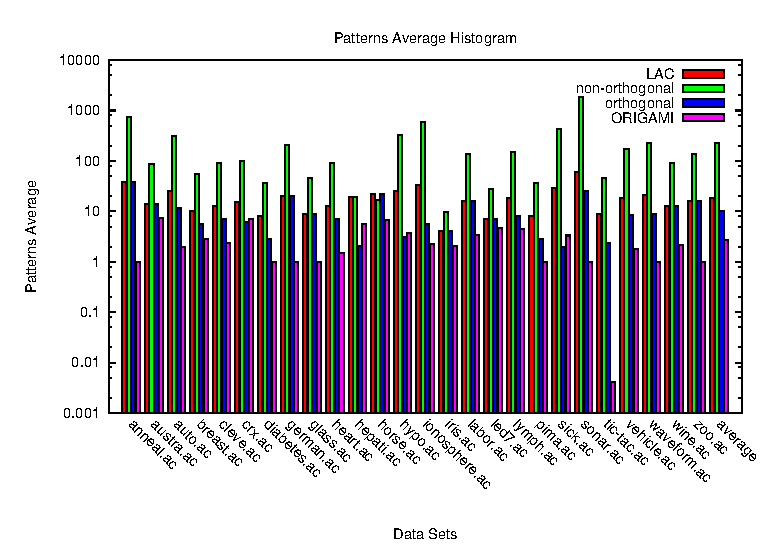
\includegraphics[width=0.95\textwidth]{graphs/histogram_best_run_for_each_db_pat}
	\caption{Histograma de Padr�es (melhores resultados para cada base de dados)}
	\label{fig:histogram_best_run_for_each_db_pat}
\end{figure}

O n�mero de padr�es gerados pelas abordagens OLAC e ORIGAMI � sempre menor ou igual ao n�mero de padr�es gerados pela abordagem LAC. Na figura \ref{fig:histogram_best_run_for_each_db_pat} vemos que, em alguns casos, as tr�s abordagens utilizam uma quantidade de padr�es freq�entes bem semelhante para gerar as regras, como na base \textit{crx.ac}. Por�m, em casos como os das bases \textit{auto.ac}, \textit{vehicle} ou \textit{waveform.ac}, a diferen�a chega a duas ou tr�s ordens de grandeza. Em m�dia, foi poss�vel reduzir o n�mero de padr�es em uma ordem de grandeza utilizando a ortogonalidade.

\begin{figure}[htbp]
	\centering
	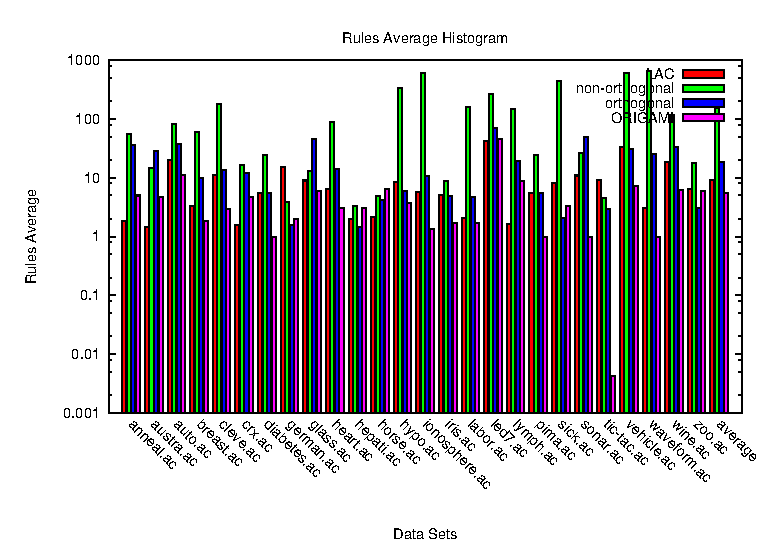
\includegraphics[width=0.95\textwidth]{graphs/histogram_best_run_for_each_db_rul}
	\caption{Histograma de Regras (melhores resultados para cada base de dados)}
	\label{fig:histogram_best_run_for_each_db_rul}
\end{figure}

O n�mero de regras geradas pelas abordagens ortogonais tamb�m se mostrou sempre menor ou igual ao n�mero de regras geradas pela abordagem n�o ortogonal, com exce��o da base \textit{hepati.ac}, em que o OLAC gerou, em m�dia, $19.78$ regras, e o LAC gerou apenas $18.43$, e das bases \textit{austra.ac} e \textit{crx.ac}, em que o ORIGAMI gerou mais regras que o LAC.
\par
� poss�vel perceber o motivo pelo qual o OLAC gerou mais regras que o LAC para a base \textit{hepati.ac} analisando as tabelas \ref{tab:best_runs_for_each_db_lac} e \ref{tab:best_runs_for_each_db_olac}. Nessas tabelas, onde temos os par�metros das melhores execu��es para cada base de dados, vemos que a melhor execu��o do LAC para esta base foi obtida com confian�a igual a $0.5$, o que reduz o n�mero de regras v�lidas consideravelmente. J� para o OLAC, a melhor execu��o para esta base foi obtida com confian�a igual a $0.0001$.
\par
A mesma observa��o � feita para o caso do ORIGAMI, analisando a tabela \ref{tab:best_runs_for_each_db_origami}. Para as bases \textit{austra.ac} e \textit{crx.ac}, a melhor execu��o do LAC foi obtida com confian�a igual a $0.3$. J� para o ORIGAMI, a confian�a foi de $0.0001$ nos dois casos.
\par
De qualquer forma, com as abordagens ortogonais foi poss�vel classificar as inst�ncias de teste com um n�mero de regras, em m�dia, dez vezes menor que com a abordagem original. Como j� era esperado, o LAC possui o menor tempo de execu��o, visto que o OLAC, al�m de obter o conjunto de padr�es freq�entes, ainda executa uma heur�stica para extrair o conjunto de padr�es ortogonais, e o ORIGAMI possui duas heur�sticas que penalizam o seu tempo de execu��o - a gera��o de padr�es maximais e a heur�stica de ortogonalidade.

\begin{figure}[htbp]
	\centering
	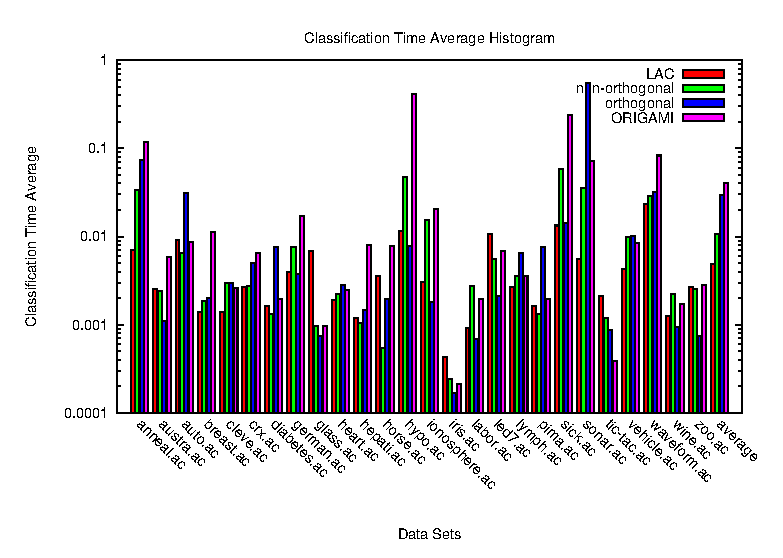
\includegraphics[width=0.95\textwidth]{graphs/histogram_best_run_for_each_db_tim}
	\caption{Histograma de Tempo (melhores resultados para cada base de dados)}
	\label{fig:histogram_best_run_for_each_db_tim}
\end{figure}

\clearpage

Como j� foi observado, na tabela \ref{tab:best_runs_for_each_db_lac} se encontram os par�metros que obtiveram as melhores acur�cias para o LAC, e os resultados de cada execu��o.

\begin{table}[htbp]
	\centering
		\begin{tabular}{|l|c|c|c|c|c|c|c|c|c|c|}
		\hline
		\textbf{dataset}	& \textbf{s}	& \textbf{c}	& \textbf{n}	& \textbf{l}	& \textbf{m}	& \textbf{x}	& \textbf{pat.}	& \textbf{rul.}	& \textbf{t.}	& \textbf{acc.}	\\
		\hline
		anneal.ac      & 0.001    & 0.7         & 1              & 1000                & 1             & 1             & 37.995         & 36.544         & 0.002          & 0.914          \\
		\hline
		austra.ac      & 0.1      & 0.8         & 1              & 100                 & 1             & 2             & 85.825         & 14.458         & 0.002          & 0.861          \\
		\hline
		auto.ac        & 0.01     & 0.8         & 1              & 10                  & 1             & 2             & 298.140        & 48.891         & 0.006          & 0.518          \\
		\hline
		breast.ac      & 0.1      & 0.0001      & 1              & 100                 & 1             & 1             & 9.661          & 19.322         & 0.001          & 0.960          \\
		\hline
		cleve.ac       & 0.0001   & 0.0001      & 1              & 100                 & 1             & 1             & 13.000         & 25.987         & 0.001          & 0.808          \\
		\hline
		crx.ac         & 0.1      & 0.8         & 1              & 1000                & 1             & 2             & 97.784         & 16.925         & 0.003          & 0.864          \\
		\hline
		diabetes.ac    & 0.01     & 0.6         & 1              & 100                 & 1             & 2             & 35.993         & 24.767         & 0.001          & 0.776          \\
		\hline
		german.ac      & 0.01     & 0.9         & 1              & 10                  & 1             & 2             & 207.909        & 3.714          & 0.007          & 0.724          \\
		\hline
		glass.ac       & 0.01     & 0.6         & 1              & 1000                & 1             & 2             & 44.884         & 12.829         & 0.001          & 0.710          \\
		\hline
		heart.ac       & 0.2      & 0.3         & 1              & 1000                & 1             & 2             & 83.326         & 118.570        & 0.002          & 0.830          \\
		\hline
		hepati.ac      & 0.1      & 0.5         & 1              & 1                   & 1             & 1             & 18.437         & 18.437         & 0.000          & 0.846          \\
		\hline
		horse.ac       & 0.3      & 0.5         & 1              & 100                 & 1             & 2             & 59.599         & 59.596         & 0.002          & 0.813          \\
		\hline
		hypo.ac        & 0.1      & 0.99        & 1              & 10                  & 1             & 2             & 290.838        & 56.591         & 0.042          & 0.978          \\
		\hline
		ionosphere.ac  & 0.01     & 0.4         & 1              & 1000                & 1             & 2             & 568.612        & 594.367        & 0.014          & 0.923          \\
		\hline
		iris.ac        & 0.1      & 0.3         & 1              & 10                  & 1             & 2             & 9.467          & 10.467         & 0.000          & 0.967          \\
		\hline
		labor.ac       & 0.3      & 0.9         & 1              & 10                  & 1             & 2             & 54.027         & 6.177          & 0.001          & 0.933          \\
		\hline
		led7.ac        & 0.1      & 0.0001      & 1              & 1000                & 1             & 2             & 27.311         & 271.501        & 0.006          & 0.729          \\
		\hline
		lymph.ac       & 0.01     & 0.5         & 1              & 1000                & 1             & 2             & 168.905        & 167.611        & 0.004          & 0.796          \\
		\hline
		pima.ac        & 0.0001   & 0.7         & 1              & 10                  & 1             & 1             & 8.000          & 3.270          & 0.000          & 0.753          \\
		\hline
		sick.ac        & 0.0001   & 0.4         & 1              & 1                   & 1             & 1             & 28.999         & 28.999         & 0.006          & 0.968          \\
		\hline
		sonar.ac       & 0.01     & 0.9         & 1              & 100                 & 1             & 2             & 1829.861       & 29.219         & 0.031          & 0.784          \\
		\hline
		tic-tac.ac     & 0.0001   & 0.5         & 1              & 1                   & 1             & 1             & 9.000          & 9.000          & 0.001          & 0.710          \\
		\hline
		vehicle.ac     & 0.0001   & 0.0001      & 1              & 100                 & 1             & 1             & 18.000         & 68.306         & 0.001          & 0.592          \\
		\hline
		waveform.ac    & 0.0001   & 0.0001      & 1              & 100                 & 1             & 1             & 21.000         & 62.912         & 0.006          & 0.765          \\
		\hline
		wine.ac        & 0.01     & 0.3         & 1              & 1000                & 1             & 2             & 90.577         & 118.375        & 0.002          & 0.994          \\
		\hline
		zoo.ac         & 0.001    & 0.7         & 1              & 1000                & 1             & 1             & 15.990         & 2.674          & 0.000          & 0.650          \\
		\hline
		\end{tabular}
	\caption{Best Parameters and Results for each Dataset (for LAC)}
	\label{tab:best_runs_for_each_db_lac}
\end{table}

\clearpage

A tabela \ref{tab:best_runs_for_each_db_olac} possui os par�metros das melhores execu��es do OLAC para cada base de dados.

\begin{table}[htbp]
	\centering
		\begin{tabular}{|l|c|c|c|c|c|c|c|c|c||c|c|c|c|}
		\hline
		\textbf{dataset}	& \textbf{s}	& \textbf{c}	& \textbf{n}	& \textbf{l}	& \textbf{m}	& \textbf{x}	& \textbf{e} & \textbf{w} & \textbf{g} & \textbf{pat.}	& \textbf{rul.}	& \textbf{t.}	& \textbf{acc.}	\\
		\hline
		anneal.ac      & 0.0001   & 0.8         & 1              & 1000                & 1             & 2             & s      & s        & s        & 21.27          & 5.64           & 0.20           & 0.92           \\
		\hline
		austra.ac      & 0.3      & 0.7         & 1              & 10                  & 1             & 2             & s      & s        & n        & 11.28          & 3.01           & 0.00           & 0.86           \\
		\hline
		auto.ac        & 0.01     & 0.4         & 1              & 10                  & 1             & 1             & s      & s        & n        & 24.25          & 12.12          & 0.00           & 0.52           \\
		\hline
		breast.ac      & 0.0001   & 0.0001      & 1              & 10                  & 1             & 2             & s      & s        & r        & 4.88           & 9.51           & 0.00           & 0.97           \\
		\hline
		cleve.ac       & 0.01     & 0.3         & 1              & 1000                & 1             & 2             & s      & s        & s        & 8.59           & 12.25          & 0.00           & 0.84           \\
		\hline
		crx.ac         & 0.3      & 0.7         & 1              & 10                  & 1             & 3             & s      & p        & n        & 12.00          & 3.00           & 0.05           & 0.86           \\
		\hline
		diabetes.ac    & 0.0001   & 0.0001      & 1              & 10                  & 1             & 2             & c      & s        & n        & 2.93           & 5.86           & 0.01           & 0.76           \\
		\hline
		german.ac      & 0.0001   & 0.8         & 1              & 1000                & 1             & 2             & s      & s        & s        & 12.35          & 1.60           & 0.02           & 0.72           \\
		\hline
		glass.ac       & 0.1      & 0.01        & 1              & 100                 & 1             & 2             & s      & s        & s        & 6.54           & 31.88          & 0.00           & 0.70           \\
		\hline
		heart.ac       & 0.01     & 0.3         & 1              & 1000                & 1             & 2             & s      & s        & s        & 8.50           & 11.95          & 0.00           & 0.83           \\
		\hline
		hepati.ac      & 0.0001   & 0.3         & 1              & 100                 & 1             & 1             & c      & s        & s        & 2.03           & 2.59           & 0.00           & 0.86           \\
		\hline
		horse.ac       & 0.3      & 0.7         & 1              & 10                  & 1             & 2             & s      & s        & n        & 13.11          & 1.29           & 0.01           & 0.81           \\
		\hline
		hypo.ac        & 0.0001   & 0.99        & 1              & 10                  & 1             & 1             & s      & p        & z        & 25.00          & 3.13           & 0.01           & 0.98           \\
		\hline
		ionosphere.ac  & 0.001    & 0.3         & 1              & 100                 & 1             & 1             & s      & s        & s        & 34.00          & 40.34          & 0.01           & 0.91           \\
		\hline
		iris.ac        & 0.01     & 0.3         & 1              & 1000                & 1             & 2             & s      & s        & s        & 3.61           & 4.32           & 0.00           & 0.97           \\
		\hline
		labor.ac       & 0.1      & 0.6         & 1              & 10                  & 1             & 2             & s      & s        & z        & 9.44           & 8.25           & 0.00           & 0.93           \\
		\hline
		led7.ac        & 0.0001   & 0.0001      & 1              & 100                 & 1             & 1             & s      & s        & s        & 7.00           & 70.00          & 0.00           & 0.63           \\
		\hline
		lymph.ac       & 0.01     & 0.6         & 1              & 10                  & 1             & 2             & s      & s        & s        & 8.79           & 4.44           & 0.01           & 0.78           \\
		\hline
		pima.ac        & 0.0001   & 0.4         & 1              & 100                 & 1             & 5             & l      & s        & r        & 4.80           & 6.11           & 0.03           & 0.76           \\
		\hline
		sick.ac        & 0.001    & 0.2         & 1              & 100                 & 1             & 2             & c      & s        & s        & 3.26           & 3.48           & 0.46           & 0.96           \\
		\hline
		sonar.ac       & 0.01     & 0.5         & 1              & 100                 & 1             & 2             & l      & s        & s        & 3.82           & 3.82           & 0.06           & 0.79           \\
		\hline
		tic-tac.ac     & 0.01     & 0.7         & 1              & 10                  & 1             & 5             & l      & s        & z        & 7.89           & 5.07           & 0.04           & 0.80           \\
		\hline
		vehicle.ac     & 0.0001   & 0.0001      & 1              & 100                 & 1             & 2             & s      & s        & z        & 8.00           & 27.95          & 0.02           & 0.64           \\
		\hline
		waveform.ac    & 0.0001   & 0.0001      & 1              & 100                 & 1             & 2             & s      & s        & r        & 9.58           & 27.32          & 0.06           & 0.79           \\
		\hline
		wine.ac        & 0.0001   & 0.0001      & 1              & 100                 & 1             & 2             & s      & s        & z        & 8.96           & 20.94          & 0.00           & 0.96           \\
		\hline
		zoo.ac         & 0.01     & 0.6         & 1              & 10                  & 1             & 2             & s      & s        & s        & 8.36           & 3.38           & 0.00           & 0.73           \\
		\hline
		\end{tabular}
	\caption{Best Parameters and Results for each Dataset (for OLAC)}
	\label{tab:best_runs_for_each_db_olac}
\end{table}

\clearpage

A tabela \ref{tab:best_runs_for_each_db_origami} possui os par�metros das melhores execu��es do ORIGAMI para cada base de dados.

\begin{table}[htbp]
	\centering
		\renewcommand{\tabcolsep}{1.8mm}
		\begin{tabular}{|l|c|c|c|c|c|c|c|c||c|c|c|c|}
		\hline
		\textbf{dataset}	& \textbf{s}	& \textbf{c}	& \textbf{n}	& \textbf{l}	& \textbf{u}	& \textbf{e} & \textbf{a} & \textbf{b} & \textbf{pat.}	& \textbf{rul.}	& \textbf{tim.}	& \textbf{acc.}	\\
		\hline
		anneal.ac      & 0.0001   & 0.0001      & 1              & 10       & c                   & s        & 0.7    & 0.9   & 1.01           & 1.01           & 0.02           & 0.96           \\
		\hline
		austra.ac      & 0.1      & 0.0001      & 1              & 100      & c                   & s        & 0.7    & 0.8   & 30.35          & 60.62          & 0.03           & 0.87           \\
		\hline
		auto.ac        & 0.1      & 0.0001      & 1              & 100      & c                   & s        & 0.7    & 0.8   & 13.47          & 51.30          & 0.02           & 0.56           \\
		\hline
		breast.ac      & 0.0001   & 0.0001      & 1              & 10       & o                   & s        & 0.1    & 0.5   & 1.00           & 1.01           & 0.00           & 0.96           \\
		\hline
		cleve.ac       & 0.1      & 0.0001      & 1              & 100      & c                   & s        & 0.7    & 0.8   & 14.76          & 28.91          & 0.01           & 0.84           \\
		\hline
		crx.ac         & 0.1      & 0.0001      & 1              & 100      & c                   & s        & 0.7    & 0.8   & 27.52          & 54.99          & 0.03           & 0.86           \\
		\hline
		diabetes.ac    & 0.1      & 0.0001      & 1              & 10       & k                   & s        & 0.7    & 0.8   & 4.49           & 8.97           & 0.00           & 0.79           \\
		\hline
		german.ac      & 0.1      & 0.0001      & 1              & 10       & e                   & c        & 0.2    & 0.8   & 8.03           & 16.05          & 0.11           & 0.73           \\
		\hline
		glass.ac       & 0.0001   & 0.0001      & 1              & 10       & c                   & s        & 0.1    & 0.5   & 1.00           & 2.00           & 0.00           & 0.77           \\
		\hline
		heart.ac       & 0.1      & 0.0001      & 1              & 10       & e                   & s        & 0.2    & 0.8   & 1.00           & 1.90           & 0.00           & 0.84           \\
		\hline
		hepati.ac      & 0.001    & 0.001       & 1              & 100      & s                   & s        & 0.1    & 0.8   & 1.00           & 1.00           & 0.00           & 0.88           \\
		\hline
		horse.ac       & 0.1      & 0.5         & 1              & 100      & c                   & s        & 0.7    & 0.8   & 53.77          & 54.63          & 0.11           & 0.79           \\
		\hline
		hypo.ac        & 0.0001   & 0.0001      & 1              & 10       & c                   & s        & 0.3    & 0.5   & 1.00           & 1.04           & 0.03           & 0.98           \\
		\hline
		ionosphere.ac  & 0.1      & 0.0001      & 1              & 100      & c                   & s        & 0.7    & 0.8   & 27.71          & 49.06          & 0.29           & 0.89           \\
		\hline
		iris.ac        & 0.1      & 0.0001      & 1              & 10       & n                   & s        & 0.2    & 0.8   & 1.06           & 1.37           & 0.00           & 0.95           \\
		\hline
		labor.ac       & 0.0001   & 0.001       & 1              & 1        & v                   & s        & 0.2    & 0.6   & 1.07           & 1.07           & 0.00           & 0.95           \\
		\hline
		led7.ac        & 0.001    & 0.0001      & 1              & 10       & c                   & l        & 0.1    & 0.4   & 1.04           & 4.56           & 0.00           & 0.73           \\
		\hline
		lymph.ac       & 0.1      & 0.001       & 1              & 100      & n                   & s        & 0.6    & 0.7   & 18.25          & 37.23          & 0.03           & 0.84           \\
		\hline
		pima.ac        & 0.1      & 0.0001      & 1              & 10       & l                   & s        & 0.7    & 0.9   & 4.52           & 9.03           & 0.00           & 0.78           \\
		\hline
		sick.ac        & 0.0001   & 0.0001      & 1              & 10       & c                   & s        & 0.2    & 0.7   & 1.00           & 1.14           & 0.03           & 0.97           \\
		\hline
		sonar.ac       & 0.1      & 0.0001      & 1              & 10       & i                   & s        & 0.2    & 0.9   & 1.00           & 1.81           & 0.32           & 0.83           \\
		\hline
		tic-tac.ac     & 0.0001   & 0.0001      & 1              & 1        & c                   & s        & 0.2    & 0.7   & 1.01           & 1.02           & 0.00           & 0.82           \\
		\hline
		vehicle.ac     & 0.0001   & 0.0001      & 1              & 10       & c                   & s        & 0.2    & 0.8   & 1.01           & 1.12           & 0.00           & 0.69           \\
		\hline
		waveform.ac    & 0.01     & 0.0001      & 1              & 100      & c                   & s        & 0.7    & 0.8   & 87.71          & 214.78         & 0.97           & 0.76           \\
		\hline
		wine.ac        & 0.0001   & 0.0001      & 1              & 1        & c                   & s        & 0.1    & 0.7   & 1.02           & 1.02           & 0.00           & 0.94           \\
		\hline
		zoo.ac         & 0.0001   & 0.6         & 1              & 10       & p                   & s        & 0.3    & 0.7   & 1.02           & 1.02           & 0.00           & 0.84           \\
		\hline
		\end{tabular}
	\caption{Melhores Par�metros e Resultados para Cada Base de Dados (ORIGAMI)}
	\label{tab:best_runs_for_each_db_origami}
\end{table}


\subsection{Melhor M�dia dos Resultados para Todas as Bases}

Na figura \ref{fig:histogram_best_run_for_avg_db_acc} se encontra o histograma com os melhores resultados para cada base de dados obtidos com LAC, OLAC e ORIGAMI. A figura  \ref{fig:histogram_best_run_for_avg_db_pat} possui um histograma com a m�dia do n�mero de padr�es utilizados por cada classifica��o, a figura \ref{fig:histogram_best_run_for_avg_db_rul} possui a m�dia do n�mero de regras obtidas em cada classifica��o, e a figura \ref{fig:histogram_best_run_for_avg_db_tim} possui a m�dia do tempo necess�rio para a classifica��o de cada inst�ncia de teste. Para teste quatro resultados foi utilizado, para cada aplica��o, o conjunto de par�metros que produziu o melhor valor m�dio de acur�cia para todo o conjunto de bases. Os conjuntos de par�metros para cada abordagem se encontram na tabela \ref{tab:best_parms_for_avg_db}, sendo que alguns deles n�o s�o aplic�veis a todas as abordagens.

\begin{table}[htbp]
	\centering
		\begin{tabular}{|l|c|c|c|}
		\hline
					& \textbf{LAC}	& \textbf{OLAC}	& \textbf{ORIGAMI}	\\
		\hline
		support			& 0.01		& 0.01		& 0.1			\\
		\hline
		confidence		& 0.6		& 0.001		& 0.0001		\\
		\hline
		min-num-rules		& 1		& 1		& 1			\\
		\hline
		max-num-rank-rules	& 1000		& 100		& 1000			\\
		\hline
		min-rule-len		& 1		& 1		& -			\\
		\hline
		max-rule-len		& 2		& 2		& -			\\
		\hline
		metric			& -		& s		& s			\\
		\hline
		method			& -		& s		& -			\\
		\hline
		pat-ordering		& -		& s		& -			\\
		\hline
		alpha			& -		& -		& 0.7			\\
		\hline
		beta			& -		& -		& 0.8			\\
		\hline
		\end{tabular}
	\caption{Best Parameters for Each Run}
	\label{tab:best_parms_for_avg_db}
\end{table}


\begin{figure}[htbp]
	\centering
	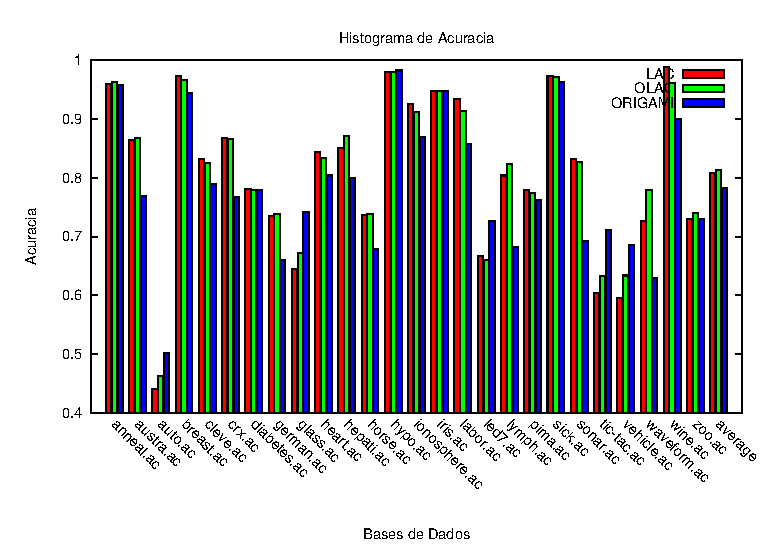
\includegraphics[width=0.95\textwidth]{graphs/histogram_best_run_for_avg_db_acc}
	\caption{Histograma de Acur�cia (m�dia dos resultados para todas as bases de dados)}
	\label{fig:histogram_best_run_for_avg_db_acc}
\end{figure}

\par
Como podemos ver, na tabela \ref{fig:histogram_best_run_for_avg_db_acc}, as melhores execu��es de cada uma das tr�s abordagens obtiveram resultados semelhantes novamente, sendo que o OLAC, dessa vez, se saiu um pouco melhor que o LAC. As m�dias obtidas para as abordagens LAC, OLAC e ORIGAMI foram, respectivamente, $0.808$, $0.813$ e $ 0.782$. � interessante notar que a melhor execu��o do OLAC foi obtida com tamanho m�ximo de regra igual a $2$ (ou seja, no m�ximo dois itens do lado esquerdo da regra), enquanto que a melhor execu��o do LAC teve tamanho m�ximo de regra igual a $1$. Isto faz com que o OLAC encontre uma quantidade de padr�es freq�entes muito maior que o LAC, no entanto, o tamanho do \textit{ranking} de regras do OLAC � menor que o do LAC, j� que a ortogonalidade diminui o n�mero de padr�es considerados durante a gera��o das regras.

\begin{figure}[htbp]
	\centering
	\includegraphics[width=0.95\textwidth]{graphs/histogram_best_run_for_avg_db_pat}
	\caption{Histograma de Padr�es (m�dia dos resultados para todas as bases de dados)}
	\label{fig:histogram_best_run_for_avg_db_pat}
\end{figure}

\par
Na tabela \ref{fig:histogram_best_run_for_avg_db_pat} vemos as quantidades de padr�es gerados por cada abordagem. A diferen�a entre os resultados obtidos com o LAC e o OLAC neste histograma n�o � t�o grande quanto no resultado anterior por influ�ncia dos par�metros de execu��o. Al�m da diferen�a entre o tamanho m�ximo das regras, que favorece o LAC \footnote{Os padr�es freq�entes utilizados pelo classificador s�o obtidos por meio de uma busca em largura no espa�o de padr�es, limitada pelo tamanho m�ximo da regra. Logo, o algoritmo s� obt�m os padr�es de tamanho menor ou igual a este par�metro}, o suporte utilizado pelo OLAC � $10$ vezes menor que o suporte do LAC.
\par
Analisando um exemplo de classifica��o podemos compreender como a utiliza��o de padr�es ortogonais pode auxiliar na classifica��o das transa��es. Para isso, usamos, como exemplo, uma configura��o de teste da base \textbf{austra.ac}. A configura��o selecionada possui $621$ transa��es de treinamento e $69$ inst�ncias de teste, das quais o OLAC classificou $61$ de maneira correta, e o LAC acertou $60$ vezes. A inst�ncia da tabela \ref{tab:table_lac_x_olac_austra.ac.test_instance_1} foi classificada corretamente pelo OLAC, mas n�o pelo LAC. Esta inst�ncia possui $14$ itens, sendo todos eles freq�entes (suporte maior que $0.0001$) na proje��o obtida, que corresponde �s $621$ transa��es da base de treinamento. Como o LAC foi executado com tamanho m�ximo das regras igual a $1$, foram encontrados $14$ padr�es freq�entes (tabela \ref{tab:table_lac_x_olac_austra.ac.lac_patterns}), com os quais foram geradas $28$ regras de associa��o com confian�a maior ou igual a $0.01$ (tabela \ref{tab:table_lac_x_olac_austra.ac.lac_rules}).

\begin{table}[htbp]
	\centering
		\renewcommand{\tabcolsep}{1.8mm}
		\begin{tabular}{|c|c|}
		\hline
		\textbf{Classe}			& \textbf{Transa��o}							\\
		\hline
		\multirow{3}{*}{CLASS=1}	& w=attr3=4.2075+ w=attr4=2 w=attr9=0 w=attr10=-0.5 w=attr11=0		\\
						& w=attr14=-493 w=attr1=1 w=attr6=4 w=attr13=99.5+ w=attr2=38.96+	\\
						& w=attr8=1 w=attr7=1.02+ w=attr5=7 w=attr12=1				\\
		\hline
		\end{tabular}
	\caption{Exemplo de Classifica��o - Inst�ncia de Teste da base \textit{austra.ac}}
	\label{tab:table_lac_x_olac_austra.ac.test_instance_1}
\end{table}

\begin{table}[htbp]
	\centering
		\renewcommand{\tabcolsep}{1.8mm}
		\begin{tabular}{|l|l|}
		\hline
		\textbf{Padr�o}	& \textbf{Suporte}	\\
		\hline		
		w=attr3=4.2075+	& 0.404187		\\
		\hline		
		w=attr4=2	& 0.756844		\\
		\hline		
		w=attr9=0	& 0.576490		\\
		\hline		
		w=attr10=-0.5	& 0.576490		\\
		\hline		
		w=attr11=0	& 0.541063		\\
		\hline		
		w=attr14=-493	& 0.764895		\\
		\hline		
		w=attr1=1	& 0.679549		\\
		\hline		
		w=attr6=4	& 0.586151		\\
		\hline		
		w=attr13=99.5+	& 0.692432		\\
		\hline		
		w=attr2=38.96+	& 0.230274		\\
		\hline		
		w=attr8=1	& 0.516908		\\
		\hline		
		w=attr7=1.02+	& 0.470209		\\
		\hline		
		w=attr5=7	& 0.054750		\\
		\hline		
		w=attr12=1	& 0.083736		\\
		\hline
		\end{tabular}
	\caption{Caso de Classifica��o - Padr�es Freq�entes Encontrados pelo LAC}
	\label{tab:table_lac_x_olac_austra.ac.lac_patterns}
\end{table}

\begin{table}[htbp]
	\centering
		\renewcommand{\tabcolsep}{1.8mm}
		\begin{tabular}{|c|l|c|}
		\hline
		\textbf{\textit{Ranking}}	& \textbf{Regra}			& \textbf{Convic��o}	\\
		\hline
		1				& CLASS=1 $\Leftarrow$ w=attr8=1		& 2.540859		\\
		\hline
		2				& CLASS=0 $\Leftarrow$ w=attr12=1	& 1.898014		\\
		\hline
		3				& CLASS=0 $\Leftarrow$ w=attr9=0		& 1.742280		\\
		\hline
		4				& CLASS=0 $\Leftarrow$ w=attr10=-0.5	& 1.742280		\\
		\hline
		5				& CLASS=1 $\Leftarrow$ w=attr7=1.02+	& 1.548142		\\
		\hline
		6				& CLASS=1 $\Leftarrow$ w=attr2=38.96+	& 1.409922		\\
		\hline
		7				& CLASS=1 $\Leftarrow$ w=attr3=4.2075+	& 1.330766		\\
		\hline
		8				& CLASS=0 $\Leftarrow$ w=attr14=-493	& 1.316782		\\
		\hline
		9				& CLASS=0 $\Leftarrow$ w=attr5=7		& 1.241009		\\
		\hline
		10				& CLASS=0 $\Leftarrow$ w=attr13=99.5+	& 1.199627		\\
		\hline
		11				& CLASS=1 $\Leftarrow$ w=attr4=2		& 1.091481		\\
		\hline
		12				& CLASS=0 $\Leftarrow$ w=attr6=4		& 1.062888		\\
		\hline
		13				& CLASS=0 $\Leftarrow$ w=attr11=0	& 1.043752		\\
		\hline
		14				& CLASS=0 $\Leftarrow$ w=attr1=1		& 1.015590		\\
		\hline
		15				& CLASS=1 $\Leftarrow$ w=attr1=1		& 0.988178		\\
		\hline
		16				& CLASS=1 $\Leftarrow$ w=attr11=0	& 0.968364		\\
		\hline
		17				& CLASS=1 $\Leftarrow$ w=attr6=4		& 0.955920		\\
		\hline
		18				& CLASS=0 $\Leftarrow$ w=attr4=2		& 0.902901		\\
		\hline
		19				& CLASS=1 $\Leftarrow$ w=attr13=99.5+	& 0.885196		\\
		\hline
		20				& CLASS=1 $\Leftarrow$ w=attr5=7		& 0.868540		\\
		\hline
		21				& CLASS=1 $\Leftarrow$ w=attr14=-493	& 0.842109		\\
		\hline
		22				& CLASS=0 $\Leftarrow$ w=attr3=4.2075+	& 0.758199		\\
		\hline
		23				& CLASS=1 $\Leftarrow$ w=attr10=-0.5	& 0.750727		\\
		\hline
		24				& CLASS=1 $\Leftarrow$ w=attr9=0		& 0.750727		\\
		\hline
		25				& CLASS=1 $\Leftarrow$ w=attr12=1	& 0.730596		\\
		\hline
		26				& CLASS=0 $\Leftarrow$ w=attr2=38.96+	& 0.728308		\\
		\hline
		27				& CLASS=0 $\Leftarrow$ w=attr7=1.02+	& 0.687618		\\
		\hline
		28				& CLASS=0 $\Leftarrow$ w=attr8=1		& 0.562396		\\
		\hline
		\end{tabular}
	\caption{Exemplo de Classifica��o - Regras de Associa��o Encontradas pelo LAC}
	\label{tab:table_lac_x_olac_austra.ac.lac_rules}
\end{table}


\par
J� o OLAC, que foi executado com tamanho m�ximo de regra igual a $2$, obteve um conjunto de $105$ padr�es freq�entes, dos quais foram extra�dos $9$ padr�es ortogonais (tabela \ref{tab:table_lac_x_olac_austra.ac.olac_patterns}), e, a partir destes, foram geradas $18$ regras com confian�a maior ou igual a $0.001$ (tabela \ref{tab:table_lac_x_olac_austra.ac.olac_rules}).

\begin{table}[htbp]
	\centering
		\renewcommand{\tabcolsep}{1.8mm}
		\begin{tabular}{|l|l|}
		\hline
		\textbf{Padr�o}			& \textbf{Suporte}	\\
		\hline		
		w=attr3=4.2075+			& 0.404187		\\
		\hline
		w=attr10=-0.5			& 0.576490		\\
		\hline
		w=attr11=0			& 0.541063		\\
		\hline
		w=attr9=0 w=attr14=-493		& 0.504026		\\
		\hline
		w=attr4=2 w=attr2=38.96+	& 0.190016		\\
		\hline
		w=attr6=4 w=attr13=99.5+	& 0.426731		\\
		\hline
		w=attr8=1 w=attr7=1.02+		& 0.334944		\\
		\hline
		w=attr1=1 w=attr5=7		& 0.049919		\\
		\hline
		w=attr12=1			& 0.083736		\\
		\hline
		\end{tabular}
	\caption{Exemplo de Classifica��o - Padr�es Freq�entes Encontrados pelo OLAC}
	\label{tab:table_lac_x_olac_austra.ac.olac_patterns}
\end{table}

\begin{table}[htbp]
	\centering
		\renewcommand{\tabcolsep}{1.8mm}
		\begin{tabular}{|c|l|c|}
		\hline
		\textbf{\textit{Ranking}}	& \textbf{Regra}				& \textbf{Convic��o}	\\
		\hline
		1				& CLASS=1 $Leftarrow$ w=attr8=1 w=attr7=1.02+	& 3.770817		\\
		\hline
		2				& CLASS=0 $Leftarrow$ w=attr9=0 w=attr14=-493	& 2.016103		\\
		\hline
		3				& CLASS=0 $Leftarrow$ w=attr12=1		& 1.898014		\\
		\hline
		4				& CLASS=0 $Leftarrow$ w=attr10=-0.5		& 1.742280		\\
		\hline
		5				& CLASS=1 $Leftarrow$ w=attr4=2 w=attr2=38.96+	& 1.617454		\\
		\hline
		6				& CLASS=1 $Leftarrow$ w=attr3=4.2075+		& 1.330766		\\
		\hline
		7				& CLASS=0 $Leftarrow$ w=attr6=4 w=attr13=99.5+	& 1.221798		\\
		\hline
		8				& CLASS=0 $Leftarrow$ w=attr1=1 w=attr5=7	& 1.131508		\\
		\hline
		9				& CLASS=0 $Leftarrow$ w=attr11=0		& 1.043752		\\
		\hline
		10				& CLASS=1 $Leftarrow$ w=attr11=0		& 0.968364		\\
		\hline
		11				& CLASS=1 $Leftarrow$ w=attr1=1 w=attr5=7	& 0.916942		\\
		\hline
		12				& CLASS=1 $Leftarrow$ w=attr6=4 w=attr13=99.5+	& 0.876054		\\
		\hline
		13				& CLASS=0 $Leftarrow$ w=attr3=4.2075+		& 0.758199		\\
		\hline
		14				& CLASS=1 $Leftarrow$ w=attr10=-0.5		& 0.750727		\\
		\hline
		15				& CLASS=1 $Leftarrow$ w=attr12=1		& 0.730596		\\
		\hline
		16				& CLASS=1 $Leftarrow$ w=attr9=0 w=attr14=-493	& 0.717980		\\
		\hline
		17				& CLASS=0 $Leftarrow$ w=attr4=2 w=attr2=38.96+	& 0.671226		\\
		\hline
		18				& CLASS=0 $Leftarrow$ w=attr8=1 w=attr7=1.02+	& 0.514716		\\
		\hline
		\end{tabular}
	\caption{Caso de Classifica��o - Regras de Associa��o Encontradas pelo OLAC}
	\label{tab:table_lac_x_olac_austra.ac.olac_rules}
\end{table}


\par
Examinando as tabelas \ref{tab:table_lac_x_olac_austra.ac.lac_rules} e \ref{tab:table_lac_x_olac_austra.ac.olac_rules}, � poss�vel perceber algumas caracter�sticas interessantes que aparecem nas regras obtidas pelo OLAC. Vemos, por exemplo, que a primeira regra do \textit{ranking}, que possui convic��o igual a $3.77$, � uma regra que contribui positivamente para o resultado correto do algoritmo, e foi obtida por meio da combina��o de dois padr�es que, na abordagem LAC, geraram regras com convic��es iguais a $2.54$ e $1.55$ respectivamente. Nota-se que a combina��o dos dois padr�es, al�m de diminuir a redund�ncia das regras, melhorou a sua medida de convic��o, fazendo com que o algoritmo se aproximasse do resultado correto.
\par
E adicionalmente, podemos perceber tamb�m que a �ltima regra do \textit{ranking} da abordagem OLAC, que possui convic��o igual a $0.51$ e contribui negativamente para o resultado, e foi obtida por meio da combina��o de duas regras da abordagem LAC com convic��es iguais a $0.69$ e $0.56$, respectivamente, ou seja, nesse caso, a medida de convic��o diminuiu. Logo, temos aqui um exemplo de como a ortogonalidade pode diminuir a redund�ncia nas informa��es obtidas, e ainda melhorar a efetividade do algoritmo.
\par
Este fato � notado com freq��ncia nos casos em que o LAC � executado com o tamanho m�ximo de regra maior que $1$, pois neste caso, o n�mero muito maior de regras ser� gerado, fazendo com haja redund�ncia tanto das regras que contribuem positivamente para o sucesso da classifica��o quanto das que contribuem negativamente. Entretanto, n�o � raro encontrar transa��es nas bases de dados que s�o definidas por um n�mero muito pequeno de padr�es, e nestes casos, a redund�ncia das regras falsas exerce maiores influ�ncias que a redund�ncia das regras verdadeiras. � justamente nestes casos que a aplica��o da ortogonalidade favorece o algoritmo.

\begin{figure}[htbp]
	\centering
	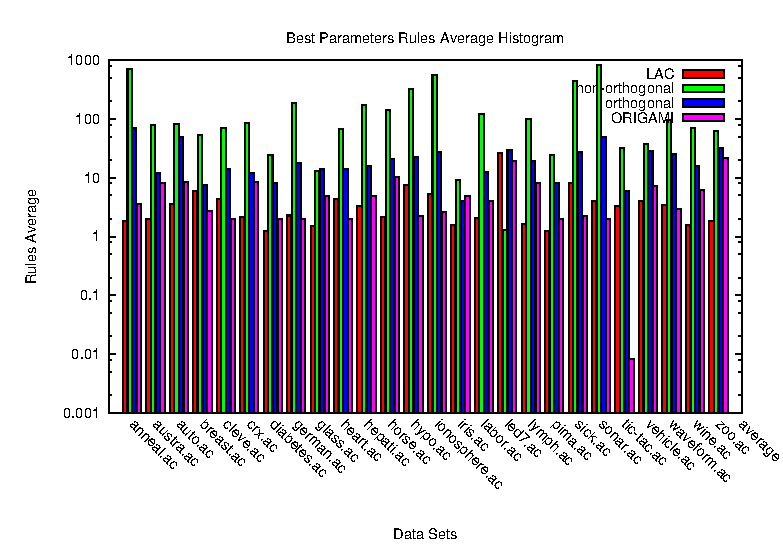
\includegraphics[width=0.95\textwidth]{graphs/histogram_best_run_for_avg_db_rul}
	\caption{Histograma de Regras (m�dia dos resultados para todas as bases de dados)}
	\label{fig:histogram_best_run_for_avg_db_rul}
\end{figure}

\par
Em rela��o ao ORIGAMI, esta abordagem obteve apenas um padr�o freq�ente e ortogonal para a maior parte das bases. Isto se deve � combina��o dos par�metros utilizados na sua melhor execu��o. Um suporte baixo favorece a gera��o de grandes padr�es maximais, que tendem a se aproximar do padr�o m�ximo obtido com todos os itens da inst�ncia de teste. Como a m�trica de ortogonalidade baseada na estrutura dos padr�es foi utilizada, isto torna dif�cil a obten��o de conjuntos ortogonais. Mesmo utilizando um valor baixo para o par�metro $\alpha$, a probabilidade de dois padr�es maximais possu�rem itens em comum � muito grande. Em grande parte dos experimentos, o tamanho m�dio dos padr�es maximais ficou bem pr�ximo do tamanho da inst�ncia de teste.
\par
Novamente, como era de se esperar, o LAC obteve o melhor desempenho das tr�s abordagens.

\begin{figure}[htbp]
	\centering
	\includegraphics[width=0.95\textwidth]{graphs/histogram_best_run_for_avg_db_tim}
	\caption{Histograma de Tempo (m�dia dos resultados para todas as bases de dados)}
	\label{fig:histogram_best_run_for_avg_db_tim}
\end{figure}

\clearpage

\subsubsection{Compara��o das M�tricas de Ortogonalidade (OLAC)}

Na figura \ref{fig:histogram_best_run_for_avg_db_ometric_acc} encontramos os valores de acur�cia obtidos por cada uma das m�tricas de ortogonalidade implementadas. Na figura \ref{fig:histogram_best_run_for_avg_db_ometric_pat} encontramos o histograma de padr�es, e em \ref{fig:histogram_best_run_for_avg_db_ometric_rul} encontramos o histograma de regras. Na figura \ref{fig:histogram_best_run_for_avg_db_ometric_tim} temos o tempo m�dio de classifica��o de uma inst�ncia de teste para cada m�trica. Todos estes resultados foram obtidos com os par�metros do OLAC encontrados na tabela \ref{tab:best_parms_for_avg_db} variando-se a m�trica de ortogonalidade.

\begin{figure}[htbp]
	\centering
	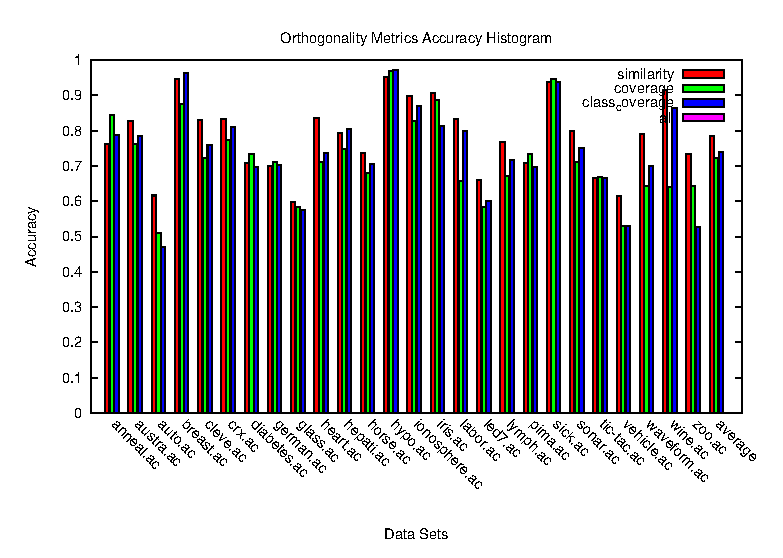
\includegraphics[width=0.95\textwidth]{graphs/histogram_best_run_for_avg_db_ometric_acc}
	\caption{Histograma de Acur�cia por M�tricas de Ortogonalidade}
	\label{fig:histogram_best_run_for_avg_db_ometric_acc}
\end{figure}

A superioridade da m�trica baseada na estrutura dos padr�es sobre as outras pode ser notada analisando a figura \ref{fig:histogram_best_run_for_avg_db_ometric_acc}. Neste experimento, a m�trica baseadas na estrutura dos padr�es encontrou conjuntos ortogonais, em geral, maiores que os encontrados pelas m�tricas baseadas em cobertura. Isto se deve, em parte, ao tamanho m�ximo das regras, que reduz o tamanho dos padr�es freq�entes considerados. Quando comparamos dois padr�es diferentes de tamanho unit�rio, a ortogonalidade ser� sempre $1$ se a m�trica baseada em estrutura for considerada. No caso das m�tricas baseadas em cobertura, este valor deve variar de acordo com a natureza dos dados. Como as aplica��es foram executadas com o limite de tamanho das regras igual a $2$, espera-se que uma boa parte do conjunto-solu��o seja composta de padr�es com apenas $1$ item.
\par
Analisando os resultados de algumas execu��es, percebemos que o problema das m�tricas baseadas em cobertura n�o est� na qualidade dos padr�es extra�dos, mas sim nas regras geradas com estes padr�es. Em grande parte das inst�ncias de teste analisadas em que a m�trica baseada em estrutura obteve sucesso, e as m�tricas baseadas em cobertura n�o obtiveram, o conjunto de padr�es ortogonais destas possu�a redund�ncia at� menor que naquele caso. Entretanto, os padr�es selecionados eram indicativos de classes diferentes das verdadeiras. Seria necess�rio um estudo mais detalhado destes casos, para ent�o chegar a uma conclus�o a respeito da utiliza��o de tais m�tricas.
\par
O tempo de execu��o do algoritmo para cada m�trica varia de acordo com a natureza da base de dados. A m�trica baseada em estrutura faz com que o desempenho do algoritmo seja influenciado pelo tamanho do conjunto de itens. J� a m�trica baseada em cobertura de transa��es faz com o que o desempenho seja influenciado pela quantidade de transa��es da base. A cobertura de classes, por sua vez, faz com que o desempenho seja influenciado pelo tamanho do conjunto de classes encontradas na base de treinamento.

\begin{figure}[htbp]
	\centering
	\includegraphics[width=0.95\textwidth]{graphs/histogram_best_run_for_avg_db_ometric_pat}
	\caption{Histograma de Padr�es por M�tricas de Ortogonalidade}
	\label{fig:histogram_best_run_for_avg_db_ometric_pat}
\end{figure}

\begin{figure}[htbp]
	\centering
	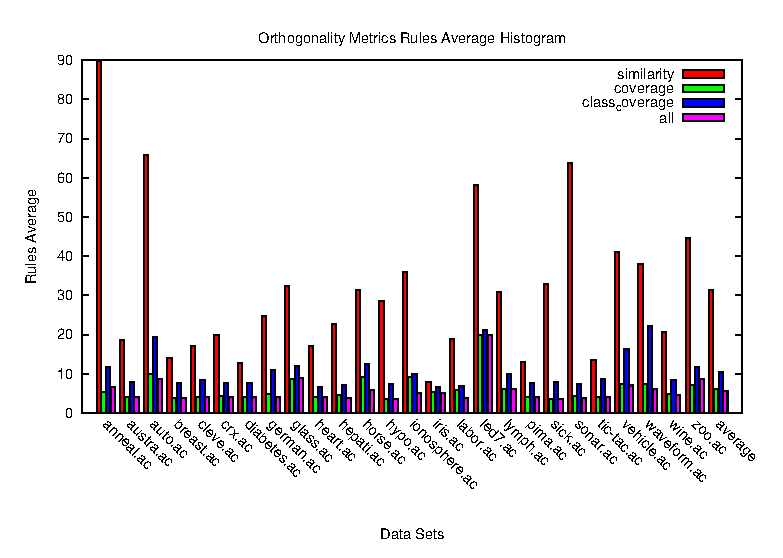
\includegraphics[width=0.95\textwidth]{graphs/histogram_best_run_for_avg_db_ometric_rul}
	\caption{Histograma de Regras por M�tricas de Ortogonalidade}
	\label{fig:histogram_best_run_for_avg_db_ometric_rul}
\end{figure}

\begin{figure}[htbp]
	\centering
	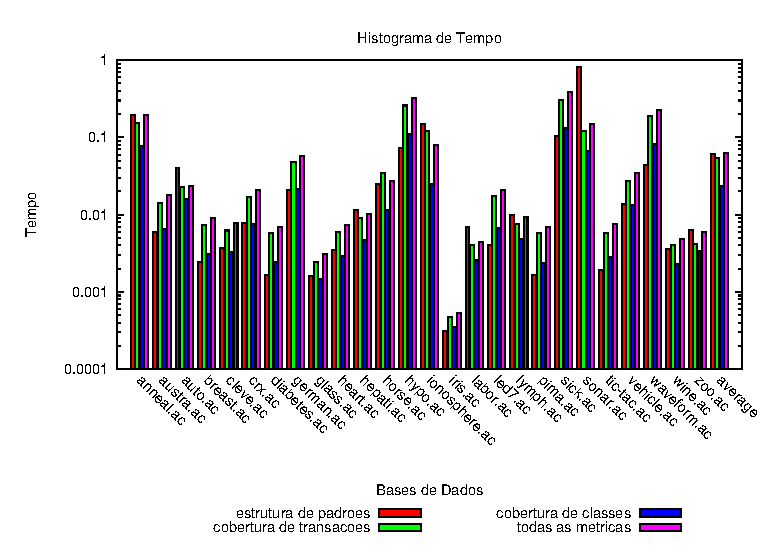
\includegraphics[width=0.95\textwidth]{graphs/histogram_best_run_for_avg_db_ometric_tim}
	\caption{Histograma de Tempo por M�tricas de Ortogonalidade}
	\label{fig:histogram_best_run_for_avg_db_ometric_tim}
\end{figure}

\clearpage

\subsubsection{Compara��o das Abordagens Quanto ao N�mero de Acertos}

Na tabela \ref{tab:comparison_lac_olac} temos uma compara��o entre as execu��es do LAC e do OLAC, onde se encontram, para cada base de dados, o n�mero de inst�ncias de teste que as duas abordagens acertaram (segunda coluna), o n�mero de inst�ncias que o OLAC acertou e o LAC errou (terceira coluna), o n�mero de inst�ncias que o LAC acertou e o OLAC errou (quarta coluna), e o n�mero de inst�ncias que as duas abordagens erraram (quinta coluna). Os resultados foram obtidos com as melhores execu��es para a m�dia de todas as bases de dados (utilizando os par�metros da tabela \ref{tab:best_parms_for_avg_db}).
\par
Com estes dados � poss�vel notar que a maioria dos acertos das duas abordagens s�o coincidentes, ou seja, a abordagem OLAC est� realizando, na maior parte das vezes, as mesmas classifica��es da abordagem LAC. A taxa de erro da estrat�gia OLAC em rela��o � quantidade de acertos total da estrat�gia LAC � de, aproximadamente, $2.3\%$, e a taxa de erro do LAC em rela��o ao OLAC � de $3.7\%$.

\begin{table}[htbp]
	\centering
		\begin{tabular}{|l|c|c|c|c|}
		\hline
				& \textbf{OLAC}		& \textbf{OLAC}			& \textbf{$\neg$ OLAC}	& \textbf{$\neg$ OLAC}	\\
		\textbf{Data Sets}	& \textbf{\&}		& \textbf{\&}			& \textbf{\&}			& \textbf{\&}			\\
				& \textbf{LAC}		& \textbf{$\neg$ LAC}		& \textbf{LAC}			& \textbf{$\neg$ LAC}		\\
		\hline
		anneal.ac       & 726           & 5                  & 3                        & 64                            \\
		\hline
		austra.ac       & 573           & 17                 & 21                       & 79                            \\
		\hline
		auto.ac         & 66            & 40                 & 40                       & 59                            \\
		\hline
		breast.ac       & 668           & 7                  & 3                        & 21                            \\
		\hline
		cleve.ac        & 239           & 16                 & 6                        & 42                            \\
		\hline
		crx.ac          & 579           & 11                 & 17                       & 83                            \\
		\hline
		diabetes.ac     & 557           & 26                 & 39                       & 146                           \\
		\hline
		german.ac       & 631           & 89                 & 93                       & 187                           \\
		\hline
		glass.ac        & 131           & 18                 & 21                       & 44                            \\
		\hline
		heart.ac        & 218           & 6                  & 6                        & 40                            \\
		\hline
		hepati.ac       & 120           & 13                 & 11                       & 11                            \\
		\hline
		horse.ac        & 298           & 0                  & 1                        & 69                            \\
		\hline
		hypo.ac         & 3083          & 2                  & 10                       & 68                            \\
		\hline
		ionosphere.ac   & 314           & 4                  & 10                       & 23                            \\
		\hline
		iris.ac         & 145           & 0                  & 0                        & 5                             \\
		\hline
		labor.ac        & 51            & 2                  & 2                        & 2                             \\
		\hline
		led7.ac         & 1988          & 39                 & 346                      & 827                           \\
		\hline
		lymph.ac        & 106           & 10                 & 12                       & 20                            \\
		\hline
		pima.ac         & 535           & 50                 & 43                       & 140                           \\
		\hline
		sick.ac         & 2631          & 49                 & 78                       & 42                            \\
		\hline
		sonar.ac        & 128           & 36                 & 35                       & 9                             \\
		\hline
		tic-tac.ac      & 601           & 167                & 79                       & 111                           \\
		\hline
		vehicle.ac      & 474           & 65                 & 27                       & 280                           \\
		\hline
		waveform.ac     & 3688          & 281                & 135                      & 896                           \\
		\hline
		wine.ac         & 171           & 0                  & 6                        & 1                             \\
		\hline
		zoo.ac          & 64            & 10                 & 2                        & 25                            \\
		\hline
		average         & 722.50        & 37.04              & 40.23                    & 126.69                        \\
		\hline
		\end{tabular}
	\caption{Comparison between LAC and OLAC (number of asserts)}
	\label{tab:comparison_lac_olac}
\end{table}

\clearpage

Na tabela \ref{tab:comparison_lac_origami} temos a compara��o entre as execu��es do LAC e do ORIGAMI. A taxa de erro do ORIGAMI em rela��o ao LAC � de $12.7\%$, e a taxa de erro do LAC em rela��o ao ORIGAMI � de $10.5\%$. Analisando os dados, vemos que a solu��o baseada na abordagem ORIGAMI se distancia um pouco mais do LAC, se compararmos com o resultado da tabela anterior. De fato, os padr�es utilizadas pelo ORIGAMI possuem caracter�sticas bem diferentes dos padr�es utilizados pelo LAC e pelo OLAC. Enquanto estes utilizam de padr�es de tamanho pequeno, o ORIGAMI utiliza apenas padr�es maximais para gerar as regras de classifica��o. Isto faz com que o comportamento do ORIGAMI seja totalmente diferente dos comportamentos do LAC e do OLAC.

\begin{table}[htbp]
	\centering
		\begin{tabular}{|l|c|c|c|c|}
		\hline
				& \textbf{ORIGAMI}	& \textbf{ORIGAMI}		& \textbf{$\neg$ ORIGAMI}	& \textbf{$\neg$ ORIGAMI}	\\
		\textbf{Data Sets}	& \textbf{\&}		& \textbf{\&}			& \textbf{\&}			& \textbf{\&}			\\
				&  \textbf{LAC}		& \textbf{$\neg$ LAC}		& \textbf{LAC}			& \textbf{$\neg$ LAC}		\\
		\hline
		anneal.ac       & 714           & 49                 & 22                       & 13                            \\
		\hline
		austra.ac       & 567           & 35                 & 27                       & 61                            \\
		\hline
		auto.ac         & 60            & 50                 & 46                       & 49                            \\
		\hline
		breast.ac       & 660           & 9                  & 18                       & 12                            \\
		\hline
		cleve.ac        & 245           & 10                 & 5                        & 43                            \\
		\hline
		crx.ac          & 562           & 32                 & 34                       & 62                            \\
		\hline
		diabetes.ac     & 560           & 41                 & 36                       & 131                           \\
		\hline
		german.ac       & 574           & 153                & 150                      & 123                           \\
		\hline
		glass.ac        & 141           & 25                 & 11                       & 37                            \\
		\hline
		heart.ac        & 213           & 13                 & 11                       & 33                            \\
		\hline
		hepati.ac       & 115           & 17                 & 16                       & 7                             \\
		\hline
		horse.ac        & 289           & 3                  & 10                       & 66                            \\
		\hline
		hypo.ac         & 3070          & 42                 & 23                       & 28                            \\
		\hline
		ionosphere.ac   & 310           & 8                  & 14                       & 19                            \\
		\hline
		iris.ac         & 140           & 3                  & 5                        & 2                             \\
		\hline
		labor.ac        & 50            & 3                  & 3                        & 1                             \\
		\hline
		led7.ac         & 2202          & 125                & 132                      & 741                           \\
		\hline
		lymph.ac        & 108           & 12                 & 10                       & 18                            \\
		\hline
		pima.ac         & 554           & 53                 & 34                       & 127                           \\
		\hline
		sick.ac         & 2675          & 45                 & 34                       & 46                            \\
		\hline
		sonar.ac        & 133           & 32                 & 30                       & 13                            \\
		\hline
		tic-tac.ac      & 584           & 204                & 96                       & 74                            \\
		\hline
		vehicle.ac      & 422           & 155                & 97                       & 172                           \\
		\hline
		waveform.ac     & 3355          & 414                & 593                      & 638                           \\
		\hline
		wine.ac         & 174           & 1                  & 3                        & 0                             \\
		\hline
		zoo.ac          & 66            & 13                 & 12                       & 10                            \\
		\hline
		average         & 713.19        & 59.50              & 56.62                    & 97.15                         \\
		\hline
		\end{tabular}
	\caption{Comparison between LAC and ORIGAMI (number of asserts)}
	\label{tab:comparison_lac_origami}
\end{table}

\clearpage

Na tabela \ref{tab:comparison_olac_origami} temos a compara��o entre as abordagens OLAC e ORIGAMI, que comprova o fato de que esta abordagem possui comportamento bem diferente daquela, fazendo com que os resultados das duas execu��es se distanciem tanto.

\begin{table}[htbp]
	\centering
		\begin{tabular}{|l|c|c|c|c|}
		\hline
				& \textbf{OLAC}		& \textbf{OLAC}			& \textbf{$\neg$ OLAC}	& \textbf{$\neg$ OLAC}	\\
		\textbf{Data Sets}	& \textbf{\&}		& \textbf{\&}			& \textbf{\&}			& \textbf{\&}			\\
				& \textbf{ORIGAMI}	& \textbf{$\neg$ ORIGAMI}	& \textbf{ORIGAMI}		& \textbf{$\neg$ ORIGAMI}	\\
		\hline
		anneal.ac       & 743           & 25                 & 21                       & 9                             \\
		\hline
		austra.ac       & 503           & 96                 & 28                       & 63                            \\
		\hline
		auto.ac         & 47            & 48                 & 56                       & 54                            \\
		\hline
		breast.ac       & 654           & 21                 & 6                        & 18                            \\
		\hline
		cleve.ac        & 216           & 34                 & 23                       & 30                            \\
		\hline
		crx.ac          & 499           & 98                 & 30                       & 63                            \\
		\hline
		diabetes.ac     & 543           & 55                 & 55                       & 115                           \\
		\hline
		german.ac       & 549           & 189                & 111                      & 151                           \\
		\hline
		glass.ac        & 132           & 12                 & 27                       & 43                            \\
		\hline
		heart.ac        & 201           & 24                 & 16                       & 29                            \\
		\hline
		hepati.ac       & 114           & 21                 & 10                       & 10                            \\
		\hline
		horse.ac        & 209           & 63                 & 41                       & 55                            \\
		\hline
		hypo.ac         & 3080          & 20                 & 27                       & 36                            \\
		\hline
		ionosphere.ac   & 289           & 31                 & 16                       & 15                            \\
		\hline
		iris.ac         & 140           & 2                  & 2                        & 6                             \\
		\hline
		labor.ac        & 46            & 6                  & 3                        & 2                             \\
		\hline
		led7.ac         & 1983          & 130                & 340                      & 747                           \\
		\hline
		lymph.ac        & 91            & 31                 & 10                       & 16                            \\
		\hline
		pima.ac         & 533           & 61                 & 52                       & 122                           \\
		\hline
		sick.ac         & 2673          & 45                 & 25                       & 57                            \\
		\hline
		sonar.ac        & 126           & 46                 & 18                       & 18                            \\
		\hline
		tic-tac.ac      & 474           & 132                & 208                      & 144                           \\
		\hline
		vehicle.ac      & 445           & 91                 & 135                      & 175                           \\
		\hline
		waveform.ac     & 2622          & 1271               & 525                      & 582                           \\
		\hline
		wine.ac         & 156           & 15                 & 4                        & 3                             \\
		\hline
		zoo.ac          & 67            & 8                  & 7                        & 19                            \\
		\hline
		average         & 659.04        & 99.04              & 69.08                    & 99.31                         \\
		\hline
		\end{tabular}
	\caption{Compara��o entre OLAC e ORIGAMI (numero de acertos)}
	\label{tab:comparison_olac_origami}
\end{table}

\subsection{Estudo de Casos de Teste}

Nesta se��o apresentaremos dois casos de teste extra�dos do \textit{log} de execu��o em que as abordagens baseadas em ortogonalidade n�o obt�m sucesso na classifica��o das inst�ncias de teste. Foram utilizados os resultados das tr�s abordagens considerando os par�metros da tabela \ref{tab:best_parms_for_avg_db}.

\subsubsection{Caso de Teste LAC x OLAC}

Ser�o apresentados, nesta se��o, os detalhes do processo de classifica��o de uma inst�ncia aleat�ria de teste em que o LAC obteve sucesso e o OLAC n�o. A configura��o selecionada possui $668$ transa��es de treinamento e $69$ inst�ncias de teste da base \textit{breast.ac}, das quais o OLAC classificou quatro de maneira errada, e o LAC, apenas duas. Ser�o apresentados os detalhes da classifica��o da inst�ncia da tabela \ref{tab:table_lac_x_olac_breast.ac.test_instance_1}. Esta inst�ncia possui $10$ itens, sendo todos eles freq�entes (suporte maior que 0.0001) na proje��o obtida, que corresponde a $630$ transa��es da base de treinamento. Visto que o LAC foi executado com tamanho m�ximo das regras igual a $1$, foram encontrados $10$ padr�es freq�entes (tabela \ref{tab:table_lac_x_olac_breast.ac.lac_patterns}), com os quais foram geradas $20$ regras de associa��o com confian�a maior ou igual a $0.01$ (tabela \ref{tab:table_lac_x_olac_breast.ac.lac_rules}).

\begin{table}[htbp]
	\centering
		\renewcommand{\tabcolsep}{1.8mm}
		\begin{tabular}{|c|c|}
		\hline
		\textbf{Classe}			& \textbf{Transa��o}							\\
		\hline
		\multirow{2}{*}{CLASS=1}	& w=attr1=ignore w=attr7=-1.5 w=attr8=-2.5 w=attr10=-1.5 w=attr5=-1.5	\\
						& w=attr9=2.5-9.5 w=attr2=6.5+ w=attr3=4.5+ w=attr4=4.5+ w=attr6=3.5+	\\
		\hline
		\end{tabular}
	\caption{Caso de Classifica��o - Inst�ncia de Teste da base \textit{breast.ac}}
	\label{tab:table_lac_x_olac_breast.ac.test_instance_1}
\end{table}

\begin{table}[htbp]
	\centering
		\renewcommand{\tabcolsep}{1.8mm}
		\begin{tabular}{|l|l|}
		\hline
		\textbf{Padr�o}	& \textbf{Suporte}	\\
		\hline		
		w=attr1=ignore	& 1.000000		\\
		\hline		
		w=attr7=-1.5	& 0.576190		\\
		\hline		
		w=attr8=-2.5	& 0.455556		\\
		\hline		
		w=attr10=-1.5	& 0.833333		\\
		\hline		
		w=attr5=-1.5	& 0.585714		\\
		\hline		
		w=attr9=2.5-9.5	& 0.226984		\\
		\hline		
		w=attr2=6.5+	& 0.212698		\\
		\hline		
		w=attr3=4.5+	& 0.247619		\\
		\hline		
		w=attr4=4.5+	& 0.260317		\\
		\hline		
		w=attr6=3.5+	& 0.268254		\\
		\hline
		\end{tabular}
	\caption{Exemplo de Classifica��o - Padr�es Freq�entes Encontrados pelo LAC}
	\label{tab:table_lac_x_olac_breast.ac.lac_patterns}
\end{table}

\begin{table}[htbp]
	\centering
		\renewcommand{\tabcolsep}{1.8mm}
		\begin{tabular}{|c|l|c|}
		\hline
		\textbf{\textit{Ranking}}	& \textbf{Regra}			& \textbf{Convic��o}	\\
		\hline
		1				& CLASS=1 $\Leftarrow$ w=attr3=4.5+	&  25.876190		\\
		\hline
		2				& CLASS=1 $\Leftarrow$ w=attr2=6.5+	&  17.781588		\\
		\hline
		3				& CLASS=0 $\Leftarrow$ w=attr8=-2.5	&  13.796825		\\
		\hline
		4				& CLASS=1 $\Leftarrow$ w=attr4=4.5+	&  13.601587		\\
		\hline
		5				& CLASS=0 $\Leftarrow$ w=attr7=-1.5	&  11.104762		\\
		\hline
		6				& CLASS=1 $\Leftarrow$ w=attr6=3.5+	&  6.595891		\\
		\hline
		7				& CLASS=0 $\Leftarrow$ w=attr5=-1.5	&  4.281774		\\
		\hline
		8				& CLASS=1 $\Leftarrow$ w=attr9=2.5-9.5	&  3.649206		\\
		\hline
		9				& CLASS=0 $\Leftarrow$ w=attr10=-1.5	&  1.497175		\\
		\hline
		10				& CLASS=0 $\Leftarrow$ w=attr1=ignore	&  1.000000		\\
		\hline
		11				& CLASS=1 $\Leftarrow$ w=attr1=ignore	&  1.000000		\\
		\hline
		12				& CLASS=1 $\Leftarrow$ w=attr10=-1.5	&  0.855856		\\
		\hline
		13				& CLASS=1 $\Leftarrow$ w=attr5=-1.5	&  0.720084		\\
		\hline
		14				& CLASS=1 $\Leftarrow$ w=attr7=-1.5	&  0.684226		\\
		\hline
		15				& CLASS=1 $\Leftarrow$ w=attr8=-2.5	&  0.680079		\\
		\hline
		16				& CLASS=0 $\Leftarrow$ w=attr9=2.5-9.5	&  0.411287		\\
		\hline
		17				& CLASS=0 $\Leftarrow$ w=attr6=3.5+	&  0.374144		\\
		\hline
		18				& CLASS=0 $\Leftarrow$ w=attr4=4.5+	&  0.353765		\\
		\hline
		19				& CLASS=0 $\Leftarrow$ w=attr2=6.5+	&  0.349551		\\
		\hline
		20				& CLASS=0 $\Leftarrow$ w=attr3=4.5+	&  0.345363		\\
		\hline
		\end{tabular}
	\caption{Caso de Classifica��o - Regras de Associa��o Encontradas pelo LAC}
	\label{tab:table_lac_x_olac_breast.ac.lac_rules}
\end{table}


\par
J� o OLAC, que foi executado com tamanho m�ximo de regra igual a $2$, obteve um conjunto de 55 padr�es freq�entes, dos quais foram extra�dos $7$ padr�es ortogonais (tabela \ref{tab:table_lac_x_olac_breast.ac.olac_patterns}), e, a partir destes, gerou $14$ regras com confian�a maior ou igual a $0.001$ (tabela \ref{tab:table_lac_x_olac_breast.ac.olac_rules}).

\begin{table}[htbp]
	\centering
		\renewcommand{\tabcolsep}{1.8mm}
		\begin{tabular}{|l|l|}
		\hline
		\textbf{Padr�o}			& \textbf{Suporte}	\\
		\hline		
		w=attr1=ignore w=attr7=-1.5	& 0.576190		\\
		\hline
		w=attr5=-1.5			& 0.585714		\\
		\hline
		w=attr9=2.5-9.5 w=attr4=4.5+	& 0.141270		\\
		\hline
		w=attr3=4.5+			& 0.247619		\\
		\hline
		w=attr2=6.5+			& 0.212698		\\
		\hline
		w=attr8=-2.5 w=attr10=-1.5	& 0.436508		\\
		\hline
		w=attr6=3.5+			& 0.268254		\\
		\hline
		\end{tabular}
	\caption{Caso de Classifica��o - Padr�es Freq�entes Encontrados pelo OLAC}
	\label{tab:table_lac_x_olac_breast.ac.olac_patterns}
\end{table}

\begin{table}[htbp]
	\centering
		\renewcommand{\tabcolsep}{1.8mm}
		\begin{tabular}{|c|l|c|}
		\hline
		\textbf{\textit{Ranking}}	& \textbf{Regra}					& \textbf{Convic��o}	\\
		\hline
		1				& CLASS=0 $\Leftarrow$ w=attr8=-2.5 w=attr10=-1.5	& 46.269840		\\
		\hline
		2				& CLASS=1 $\Leftarrow$ w=attr3=4.5+			& 25.876190		\\
		\hline
		3				& CLASS=1 $\Leftarrow$ w=attr2=6.5+			& 17.781588		\\
		\hline
		4				& CLASS=0 $\Leftarrow$ w=attr1=ignore w=attr7=-1.5	& 11.104762		\\
		\hline
		5				& CLASS=1 $\Leftarrow$ w=attr9=2.5-9.5 w=attr4=4.5+	& 8.435827		\\
		\hline
		6				& CLASS=1 $\Leftarrow$ w=attr6=3.5+			& 6.595891		\\
		\hline
		7				& CLASS=0 $\Leftarrow$ w=attr5=-1.5			& 4.281774		\\
		\hline
		8				& CLASS=1 $\Leftarrow$ w=attr5=-1.5			& 0.720084		\\
		\hline
		9				& CLASS=1 $\Leftarrow$ w=attr1=ignore w=attr7=-1.5	& 0.684226		\\
		\hline
		10				& CLASS=1 $\Leftarrow$ w=attr8=-2.5 w=attr10=-1.5	& 0.668353		\\
		\hline
		11				& CLASS=0 $\Leftarrow$ w=attr6=3.5+			& 0.374144		\\
		\hline
		12				& CLASS=0 $\Leftarrow$ w=attr9=2.5-9.5 w=attr4=4.5+	& 0.365234		\\
		\hline
		13				& CLASS=0 $\Leftarrow$ w=attr2=6.5+			& 0.349551		\\
		\hline
		14				& CLASS=0 $\Leftarrow$ w=attr3=4.5+			& 0.345363		\\
		\hline
		\end{tabular}
	\caption{Caso de Classifica��o - Regras de Associa��o Encontradas pelo OLAC}
	\label{tab:table_lac_x_olac_breast.ac.olac_rules}
\end{table}


\par
Analisando as tabelas \ref{tab:table_lac_x_olac_breast.ac.lac_patterns} e \ref{tab:table_lac_x_olac_breast.ac.olac_patterns}, percebe-se que todos os itens da inst�ncia de teste s�o encontrados nos conjuntos de padr�es freq�entes das duas execu��es. No caso do LAC, j� era esperado que cada item correspondesse a um padr�o, pelo fato de todos os itens serem freq�entes. Em rela��o ao OLAC, era esperado um sub-conjunto dos padr�es freq�entes com baixa redund�ncia em rela��o ao conjunto original. Como o OLAC foi executado com tamanho m�ximo de regra igual a 2, o conjunto de padr�es freq�entes encontrados foi bem maior que o mesmo conjunto obtido pela estrat�gia LAC, por�m, nota-se que o conjunto de padr�es ortogonais � menor, mesmo cobrindo todos os itens da inst�ncia de teste. Al�m disso, nenhum item foi utilizado mais de uma vez, o que comprova a baixa redund�ncia do conjunto.
\par
Entretanto, apesar da boa qualidade do conjunto de padr�es ortogonais encontrado, a classifica��o n�o foi realizada com sucesso pelo OLAC. Uma an�lise simples das tabelas \ref{tab:table_lac_x_olac_breast.ac.lac_rules} e \ref{tab:table_lac_x_olac_breast.ac.olac_rules} � suficiente para entender o motivo deste erro. Na primeira tabela, vemos que as regras que mais contribuem para a classifica��o correta aparecem no topo do \textit{ranking} (posi��es 1, 2 e 4), com medidas de convic��o grandes o suficiente para que a escolha da classe correta seja realizada. A m�dia das convic��es das regras que apontam para a classe \textbf{CLASS=1} � $7.14$, enquanto que, para a classe \textbf{CLASS=0}, este valor � igual a $3.35$. J� na segunda tabela, nota-se a presen�a de regras que contribuem para a classifica��o falsa numa propor��o pr�xima � das regras verdadeiras. A primeira regra do \textit{ranking}, que possui o padr�o \textbf{w=attr8=-2.5 w=attr10=-1.5} e aponta para a  classe \textbf{CLASS=0}, � respons�vel pela maior contribui��o para o erro da classifica��o, com a medida de convic��o igual a $46.27$. Na primeira tabela, vemos que os padr�es \textbf{w=attr8=-2.5} e \textbf{w=attr10=-1.5} tamb�m contribuem para a classe falsa, mas com convic��es iguais a $13.80$ e $11.10$, respectivamente. O que acontece, neste caso, � que existe uma rela��o entre o padr�o \textbf{w=attr8=-2.5 w=attr10=-1.5} e a classe \textbf{CLASS=0} muito maior que a rela��o entre os sub-padr�es \textbf{w=attr8=-2.5} e \textbf{w=attr10=-1.5} e a classe \textbf{CLASS=0}. Isto fez com que a m�dia das regras que apontam para a classe \textbf{CLASS=0} ficasse em $9.01$, enquanto que a m�dia da classe \textbf{CLASS=1} ficou em $8.68$.
\par
Um caso semelhante ocorre tamb�m com a segunda inst�ncia classificada de maneira errada pelo OLAC, onde o padr�o \textbf{w=attr9=2.5-9.5 w=attr7=?}, por n�o fazer parte de nenhuma transa��o de classe \textbf{CLASS=0} na proje��o, obteve uma medida infinita de convic��o, fazendo com que esta classe fosse escolhida como resultado, onde o correto seria escolher a classe \textbf{CLASS=1}.
\par
Situa��es desse tipo contribu�ram para que a abordagem OLAC n�o classificasse corretamente todas as inst�ncias em que a abordagem LAC obteve sucesso. No entanto, os erros encontrados est�o mais relacionados com a natureza dos dados do que com o conceito de ortogonalidade.

\subsubsection{Caso de Teste LAC x ORIGAMI}

Nesta se��o comparamos o comportamento do LAC e do ORIGAMI no processo de classifica��o de uma inst�ncia aleat�ria de teste em que o LAC obteve sucesso e o ORIGAMI n�o. A configura��o selecionada possui $52$ transa��es de treinamento e $5$ inst�ncias de teste da base \textit{labor.ac}, das quais o ORIGAMI classificou $2$ de maneira correta, e o LAC n�o errou nenhuma classifica��o. A inst�ncia escolhida se encontra na tabela \ref{tab:table_lac_x_origami_labor.ac.test_instance_1}. Esta inst�ncia possui $16$ itens, sendo todos eles freq�entes na proje��o obtida, que corresponde �s $52$ transa��es da base de treinamento. Assim como no exemplo anterior, cada item da inst�ncia de teste deu origem a um padr�o freq�ente (tabela \ref{tab:table_lac_x_origami_labor.ac.lac_patterns}), com os quais foram obtidas $31$ regras de associa��o com confian�a maior ou igual a $0.01$ (tabela \ref{tab:table_lac_x_origami_labor.ac.lac_rules}).

\begin{table}[htbp]
	\centering
		\renewcommand{\tabcolsep}{1.8mm}
		\resizebox{0.95\textwidth}{!} {
		\begin{tabular}{|c|c|}
		\hline
		\textbf{Classe}			& \textbf{Transa��o}							\\
		\hline
		\multirow{4}{*}{CLASS=0}	& w=attr1=ignore w=attr3=-3.25 w=attr4=? w=attr6=ignore w=attr8=?	\\
						& w=attr9=? w=attr11=ignore w=attr13=? w=attr14=? w=attr2=2.65+		\\
						& w=attr7=? w=attr15=yes w=attr10=yes w=attr5=none w=attr16=full	\\
						& w=attr12=generous							\\
		\hline
		\end{tabular}
		}
	\caption{Exemplo de Classifica��o - Inst�ncia de Teste da base \textit{labor.ac}}
	\label{tab:table_lac_x_origami_labor.ac.test_instance_1}
\end{table}

\begin{table}[htbp]
	\centering
		\renewcommand{\tabcolsep}{1.8mm}
		\begin{tabular}{|l|l|}
		\hline
		\textbf{Padr�o}		& \textbf{Suporte}	\\
		\hline		
		w=attr1=ignore		& 0.980769		\\
		w=attr3=-3.25		& 0.211538		\\
		w=attr4=?		& 0.730769		\\
		w=attr6=ignore		& 0.884615		\\
		w=attr8=?		& 0.846154		\\
		w=attr9=?		& 0.461538		\\
		w=attr11=ignore		& 0.923077		\\
		w=attr13=?		& 0.519231		\\
		w=attr14=?		& 0.346154		\\
		w=attr2=2.65+		& 0.711538		\\
		w=attr7=?		& 0.519231		\\
		w=attr15=yes		& 0.461538		\\
		w=attr10=yes		& 0.153846		\\
		w=attr5=none		& 0.365385		\\
		w=attr16=full		& 0.288462		\\
		w=attr12=generous	& 0.250000		\\
		\hline
		\end{tabular}
	\caption{Exemplo de Classifica��o - Padr�es Freq�entes Encontrados pelo LAC}
	\label{tab:table_lac_x_origami_labor.ac.lac_patterns}
\end{table}


\begin{table}[htbp]
	\centering
		\renewcommand{\tabcolsep}{1.8mm}
		\begin{tabular}{|c|l|c|}
		\hline
		\textbf{\textit{Ranking}}	& \textbf{Regra}				& \textbf{Convic��o}	\\
		\hline
		1				& CLASS=0 $\Leftarrow$ w=attr7=?		& 0.925926		\\ 
		\hline
		2				& CLASS=0 $\Leftarrow$ w=attr12=generous	& 0.923077		\\ 
		\hline
		3				& CLASS=1 $\Leftarrow$ w=attr3=-3.25		& 0.818182		\\ 
		\hline
		4				& CLASS=0 $\Leftarrow$ w=attr2=2.65+		& 0.837838		\\ 
		\hline
		5				& CLASS=0 $\Leftarrow$ w=attr10=yes		& 0.750000		\\ 
		\hline
		6				& CLASS=0 $\Leftarrow$ w=attr13=?		& 0.740741		\\ 
		\hline
		7				& CLASS=0 $\Leftarrow$ w=attr16=full		& 0.733333		\\ 
		\hline
		8				& CLASS=0 $\Leftarrow$ w=attr15=yes		& 0.708333		\\ 
		\hline
		9				& CLASS=1 $\Leftarrow$ w=attr5=none		& 0.421053		\\ 
		\hline
		10				& CLASS=1 $\Leftarrow$ w=attr9=?		& 0.416667		\\ 
		\hline
		11				& CLASS=0 $\Leftarrow$ w=attr8=?		& 0.681818		\\ 
		\hline
		12				& CLASS=1 $\Leftarrow$ w=attr4=?		& 0.394737		\\ 
		\hline
		13				& CLASS=1 $\Leftarrow$ w=attr11=ignore		& 0.375000		\\ 
		\hline
		14				& CLASS=0 $\Leftarrow$ w=attr14=?		& 0.666667		\\ 
		\hline
		15				& CLASS=1 $\Leftarrow$ w=attr6=ignore		& 0.369565		\\ 
		\hline
		16				& CLASS=1 $\Leftarrow$ w=attr1=ignore		& 0.352941		\\ 
		\hline
		17				& CLASS=0 $\Leftarrow$ w=attr1=ignore		& 0.647059		\\ 
		\hline
		18				& CLASS=1 $\Leftarrow$ w=attr14=?		& 0.333333		\\ 
		\hline
		19				& CLASS=1 $\Leftarrow$ w=attr8=?		& 0.318182		\\ 
		\hline
		20				& CLASS=0 $\Leftarrow$ w=attr6=ignore		& 0.630435		\\ 
		\hline
		21				& CLASS=0 $\Leftarrow$ w=attr11=ignore		& 0.625000		\\ 
		\hline
		22				& CLASS=1 $\Leftarrow$ w=attr15=yes		& 0.291667		\\ 
		\hline
		23				& CLASS=1 $\Leftarrow$ w=attr16=full		& 0.266667		\\ 
		\hline
		24				& CLASS=1 $\Leftarrow$ w=attr13=?		& 0.259259		\\ 
		\hline
		25				& CLASS=0 $\Leftarrow$ w=attr4=?		& 0.605263		\\ 
		\hline
		26				& CLASS=1 $\Leftarrow$ w=attr10=yes		& 0.250000		\\ 
		\hline
		27				& CLASS=0 $\Leftarrow$ w=attr9=?		& 0.583333		\\ 
		\hline
		28				& CLASS=0 $\Leftarrow$ w=attr5=none		& 0.578947		\\ 
		\hline
		29				& CLASS=1 $\Leftarrow$ w=attr2=2.65+		& 0.162162		\\ 
		\hline
		30				& CLASS=1 $\Leftarrow$ w=attr12=generous	& 0.076923		\\ 
		\hline
		31				& CLASS=1 $\Leftarrow$ w=attr7=?		& 0.074074		\\ 
		\hline
		32				& CLASS=0 $\Leftarrow$ w=attr3=-3.25		& 0.181818		\\ 
		\hline
		\end{tabular}
	\caption{Caso de Classifica��o - Regras de Associa��o Encontradas pelo LAC}
	\label{tab:table_lac_x_origami_labor.ac.lac_rules}
\end{table}


\par
O ORIGAMI, por sua vez, obteve um conjunto de $13$ padr�es maximais, que se encontram na tabela \ref{tab:table_lac_x_origami_labor.ac.origami_patterns}, de onde foi extra�do um �nico padr�o ortogonal, e, posteriormente, a �nica regra de associa��o com confian�a maior ou igual a $0.0001$, que pode ser vista na tabela \ref{tab:table_lac_x_origami_labor.ac.origami_rules}. � importante notar que todos os padr�es maximais obtidos possuem suporte igual a $0.019231$, o que corresponde � fra��o $\frac{1}{52}$, ou seja, nenhum padr�o maximal obtido aparece em mais de uma transa��o na base de dados. A combina��o de par�metros de execu��o utilizada foi respons�vel por fazer com que o algoritmo n�o selecionasse uma maior quantidade de padr�es ortogonais. Como o valor do par�metro $\alpha$ utilizado foi muito baixo ($0.1$), e o suporte utilizado favoreceu a obten��o de grandes padr�es maximais, a m�trica de ortogonalidade por estrutura de padr�es n�o foi adequada. Isso aconteceu porque todos os padr�es encontrados possuem similaridade maior que $10\%$, pelo fato de v�rios itens aparecerem em mais de um padr�o. Os itens \textbf{w=attr1=ignore} e \textbf{w=attr8=?}, por exemplo, est�o presentes em todos os padr�es.
\par
Assim, a �nica regra obtida pela abordagem ORIGAMI aponta para a classe \textbf{CLASS=1}, fazendo com que o algoritmo classifique a inst�ncia de teste de maneira errada.

\begin{table}[htbp]
	\centering
		\renewcommand{\tabcolsep}{1.8mm}
		\resizebox{0.95\textwidth}{!} {
		\begin{tabular}{|l|c|}
		\hline
		\textbf{Padr�o}									& \textbf{Suporte}		\\
		\hline		
		w=attr1=ignore w=attr6=ignore w=attr8=? w=attr9=? w=attr11=ignore		& \multirow{3}{*}{0.019231}	\\
		w=attr13=? w=attr14=? w=attr2=2.65+ w=attr7=? w=attr15=yes w=attr16=full	&				\\
		w=attr12=generous								& 				\\
		\hline
		w=attr1=ignore w=attr3=-3.25 w=attr4=? w=attr6=ignore w=attr8=?			& \multirow{2}{*}{0.019231}	\\
		w=attr11=ignore	w=attr13=? w=attr14=? w=attr7=? w=attr10=yes			&				\\
		\hline
		w=attr1=ignore w=attr3=-3.25 w=attr4=? w=attr8=? w=attr9=? w=attr15=yes		& \multirow{2}{*}{0.019231}	\\
		w=attr10=yes									&				\\
		\hline
		w=attr1=ignore w=attr3=-3.25 w=attr6=ignore w=attr8=? w=attr9=?			& \multirow{2}{*}{0.019231}	\\
		w=attr11=ignore w=attr13=? w=attr15=yes w=attr5=none w=attr16=full		&				\\
		\hline
		w=attr1=ignore w=attr3=-3.25 w=attr4=? w=attr6=ignore w=attr8=? w=attr9=?	& \multirow{2}{*}{0.019231}	\\
		w=attr11=ignore w=attr13=? w=attr14=? w=attr15=yes w=attr16=full		&				\\
		\hline
		w=attr1=ignore w=attr6=ignore w=attr8=? w=attr11=ignore w=attr13=?		& \multirow{3}{*}{0.019231}	\\
		w=attr14=? w=attr2=2.65+ w=attr7=? w=attr15=yes w=attr5=none			&				\\
		w=attr16=full w=attr12=generous							&				\\
		\hline
		w=attr1=ignore w=attr4=? w=attr6=ignore w=attr8=? w=attr11=ignore		& \multirow{2}{*}{0.019231}	\\
		w=attr13=? w=attr2=2.65+ w=attr7=? w=attr16=full w=attr12=generous		&				\\
		\hline
		w=attr1=ignore w=attr8=? w=attr9=? w=attr13=? w=attr14=? w=attr2=2.65+		& \multirow{2}{*}{0.019231}	\\
		w=attr7=? w=attr15=yes w=attr10=yes						&				\\
		\hline
		w=attr1=ignore w=attr4=? w=attr6=ignore w=attr8=? w=attr11=ignore		& \multirow{2}{*}{0.019231}	\\
		w=attr13=? w=attr14=? w=attr2=2.65+ w=attr7=? w=attr15=yes			&				\\
		\hline
		w=attr1=ignore w=attr3=-3.25 w=attr4=? w=attr6=ignore w=attr8=? w=attr9=?	& \multirow{2}{*}{0.019231}	\\
		w=attr11=ignore w=attr15=yes w=attr5=none w=attr16=full				&				\\
		\hline
		w=attr1=ignore w=attr4=? w=attr6=ignore w=attr8=? w=attr9=?			& \multirow{2}{*}{0.019231}	\\
		w=attr11=ignore w=attr2=2.65+ w=attr15=yes w=attr5=none w=attr16=full		&				\\
		\hline
		w=attr1=ignore w=attr4=? w=attr6=ignore w=attr8=? w=attr11=ignore		& \multirow{3}{*}{0.019231}	\\
		w=attr13=? w=attr2=2.65+ w=attr7=? w=attr15=yes w=attr5=none			&				\\
		w=attr16=full									&				\\
		\hline
		w=attr1=ignore w=attr4=? w=attr8=? w=attr9=? w=attr11=ignore			& \multirow{2}{*}{0.019231}	\\
		w=attr2=2.65+ w=attr7=? w=attr10=yes						&				\\
		\hline
		\end{tabular}
		}
	\caption{Exemplo de Classifica��o - Padr�es Freq�entes Encontrados pelo ORIGAMI}
	\label{tab:table_lac_x_origami_labor.ac.origami_patterns}
\end{table}

\begin{table}[htbp]
	\centering
		\renewcommand{\tabcolsep}{1.8mm}
		\begin{tabular}{|c|l|c|}
		\hline
		\textbf{\textit{Ranking}}	& \textbf{Regra}			& \textbf{Confian�a}	\\
		\hline

		\multirow{3}{*}{1}		& CLASS=1 $\Leftarrow$ w=attr1=ignore w=attr3=-3.25 w=attr6=ignore	& \multirow{3}{*}{1.000000}	\\
						& w=attr8=? w=attr9=? w=attr11=ignore w=attr13=? w=attr15=yes		&				\\
						& w=attr5=none w=attr16=full						& 				\\
		\hline
		\end{tabular}
	\caption{Caso de Classifica��o - Regras de Associa��o Encontradas pelo ORIGAMI}
	\label{tab:table_lac_x_origami_labor.ac.origami_rules}
\end{table}


\chapter{Conclus�o}

\section{Resumo}
\section{Trabalhos Futuros}


\ufmgbibliography{thesis}

\end{document}
